\chapter{Digital Calorimetry}
\label{sect:DECAL}

\section{Introduction}
As mentioned in \refsec{det:ecal}, several alternatives exist for the \ac{ECAL} design of \ac{ILD}. Here we present details of a proposed fully digital \ac{ECAL} that simply counts the number of pixels above threshold rather than measuring the energy deposited in each pixel. This works based on the fact that the number of particles produced by an electromagnetic shower is proportional to the energy of the incident particle producing it.

The digital approach has several potential benefits. Fundamentally it should allow for a slight improvement in the energy resolution as it is less senstive to uncertainties arising from landau fluctuations and varying path lengths as the particle traverses the active material. In order to observe every particle within a shower any choice of \ac{DECAL} technology must have an extremely high granularity ($\mathcal{O}$(50$\mu m$)). This ultra high granularity has the potential to improve the performance of particle flow algorithms by allowing for better patern recognition and association of tracks to \ac{ECAL} deposits. Lastly, as will be discussed below, the natural choice of technology will be to use \ac{CMOS} \ac{MAPS}. As this is the same technology as is proposed for the inner tracking systems this would allow a uniform technology solution to be used across multiple detector components. It is also a cheaper technology option than that used by the alternative \ac{ECAL} designs due to the prevalence of \ac{CMOS} in commercial products.

While the digital option provides these benefits it does come with one potential flaw referred to as saturation. In a digital calorimeter, if two particles pass through the same pixel, only one hit will be registered and so the total number of particles in the shower (and thus the energy of the shower) will be underestimated. The density of an EM shower scales according to the energy of the showering particle. As a result the rate of multiple occupancy in the pixels will increase with energy leading to a non linear relationship between a particles energy and the number of hits it generates within the detector. In practice this problem can be avoided by ensuring that the granularity of the detector is always greater than the density of the electromagnetic showers. For typical \ac{ILC} energies the density of the showers is estimated to be $\mathcal{O}$ 100 particles/mm$^2$ and so a granularity of at least 50$\times$50~$\mu$m$^2$ is required to ensure only one particle hits each pixel. Note that in the analogue case this problem does not occur as the energy deposited in the pixel is what is measured and this scales with the number of particles passing through the pixel.

\begin{figure}
  \centering
  \begin{subfigure}[t]{.45\textwidth}
    \centering
    
\includegraphics[width=1\linewidth,keepaspectratio]{DECALStudies/fig/cmos_3Tdesign}
  \end{subfigure}%%%
  \begin{subfigure}[t]{.45\textwidth}
    \centering
    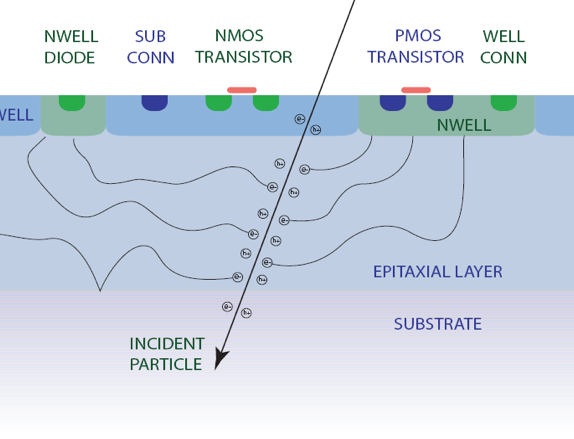
\includegraphics[width=1\linewidth,keepaspectratio]{DECALStudies/fig/nodeeppwell}
  \end{subfigure}
  \caption{Left: Schematic of the simplest layout for a \ac{CMOS} sensor using just three transistors. The first transistor, M$_{rst}$, acts as a switch to reset the charge collected at the diode. M$_{SF}$ allows the charge of the diode to be measured and amplified without removing the charge. Finally M$_{Sel}$ controls when the signal is read out from the pixel. Right: physical layout of a typical \ac{CMOS} pixel sensor.}
  \label{fig:cmosdesign}
\end{figure}

The requirement on the granularity is what ultimately leads to the decision to use a \ac{MAPS} based technology. For \ac{ILD}, using 50$\times$50~$\mu$m$^2$ pixels requires the use of $\mathcal{O}$(10$^{12}$) pixels. Having separate readout electronics, along with cooling and power supplies for each cell becomes impractical and produces large dead space within the detector. By using \ac{MAPS} technology the electronics can instead be integrated into the silicon of the pixels leading to a more compact structure. \ac{CMOS} is then chosen as it is a cheap, well understood and commercial process for producing \ac{MAPS} structures. The typical layout of a \ac{CMOS} \ac{MAPS} pixel is shown in \reffig{fig:cmosdesign}. In practice this simple design is found to be unsatisfactory for use in particle physics due to the low signal yield due to parasitic losses to the PMOS transistor. A process referred to as INMAPS was developed at \ac{RAL}\cite{2008arXiv0807.2920B} which uses the addition of a deep p well around the PMOS transistor to mitigate the signal loss. The layout of this variation is shown in \reffig{fig:deeppwell}. Two sensors based on the deep p well design have already been produced (TPAC\cite{Ballin:2008rha} and CHERWELL\cite{MYLROIESMITH2013137}) and used to show the validity of this approach for producing a \ac{DECAL}\cite{Price:2013js}. In both cases the test pixels were based on a 50$\times$50~$\mu$m$^2$ design.


\begin{figure}
  \centering
  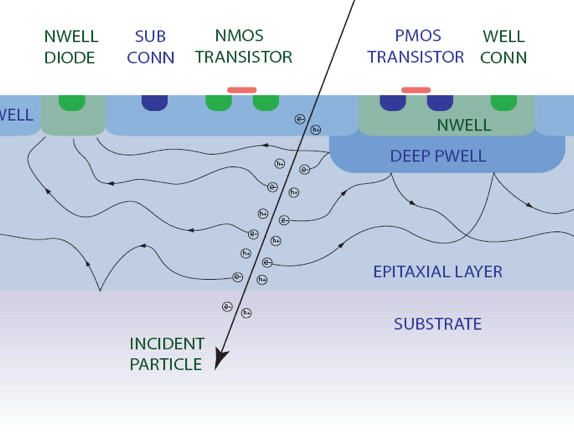
\includegraphics[width=0.5\textwidth,keepaspectratio]{DECALStudies/fig/deeppwell}
  \caption{\ac{CMOS} \ac{MAPS} sensor including deep p well implant to prevent parastic losses to the PMOS transistor\cite{MYLROIESMITH2013137}}
  \label{fig:deeppwell}
\end{figure}

Here we will present simulation studies looking at the optimization of the pixel dimensions for the sensors when including variation levels of realism such as noise, deadspace and clustering.  

\section{Event Generation and Detector Simulation}


Simulation of the \ac{DECAL} was performed in the GEANT4 based ILCSoft application, Mokka v08-05. The model used was based on an existing model for \ac{ILD}, ILD\_v01\_05, and so includes the high level of detail implemented for the \ac{ILD} letter of intent studies\cite{ILD} e.g. realistic geometries including support structures. The design was then adapated in three main ways. Firstly, the 300~$\mu$m thick active layer of silicon is divided into a thin active epitaxial layer (10-20~$\mu$m) and a deeper passive layer of silicon (280-290~$\mu$m.) The thin active layer represents what would be used in a typical \ac{CMOS} \ac{MAPS} sensor while the deeper passive layer is only included to prevent the need for changing the detailed layer structure of the exisiting model. In practice such a deep passive silicon layer would not be used. Secondly, the pixel pitch was reduced down to 5$\times$5~$\mu$m$^2$. This is smaller than can realistically be manufactured at present, however by using a narrow pixel pitch during the simulation the pixels can later be grouped together into larger virtual pixels with realistic dimensions preventing the need for simulating events at every pixel pitch required for the study and saving considerable processing time. The final change implemented was to remove the guard ring structures present in the analogue design. In the analogue design the guard rings are 1 mm metal rings placed around wafers of 18$\times$18 pixels. For the digital case these structures are not required and would result in a large amount of dead space in the detector due to the considerabley narrower pixel pitch. On top of this the magnetic field present for \ac{ILD} was turned off so that only the intrinsic \ac{ECAL} performance would be measured.

\begin{figure}
  \centering
  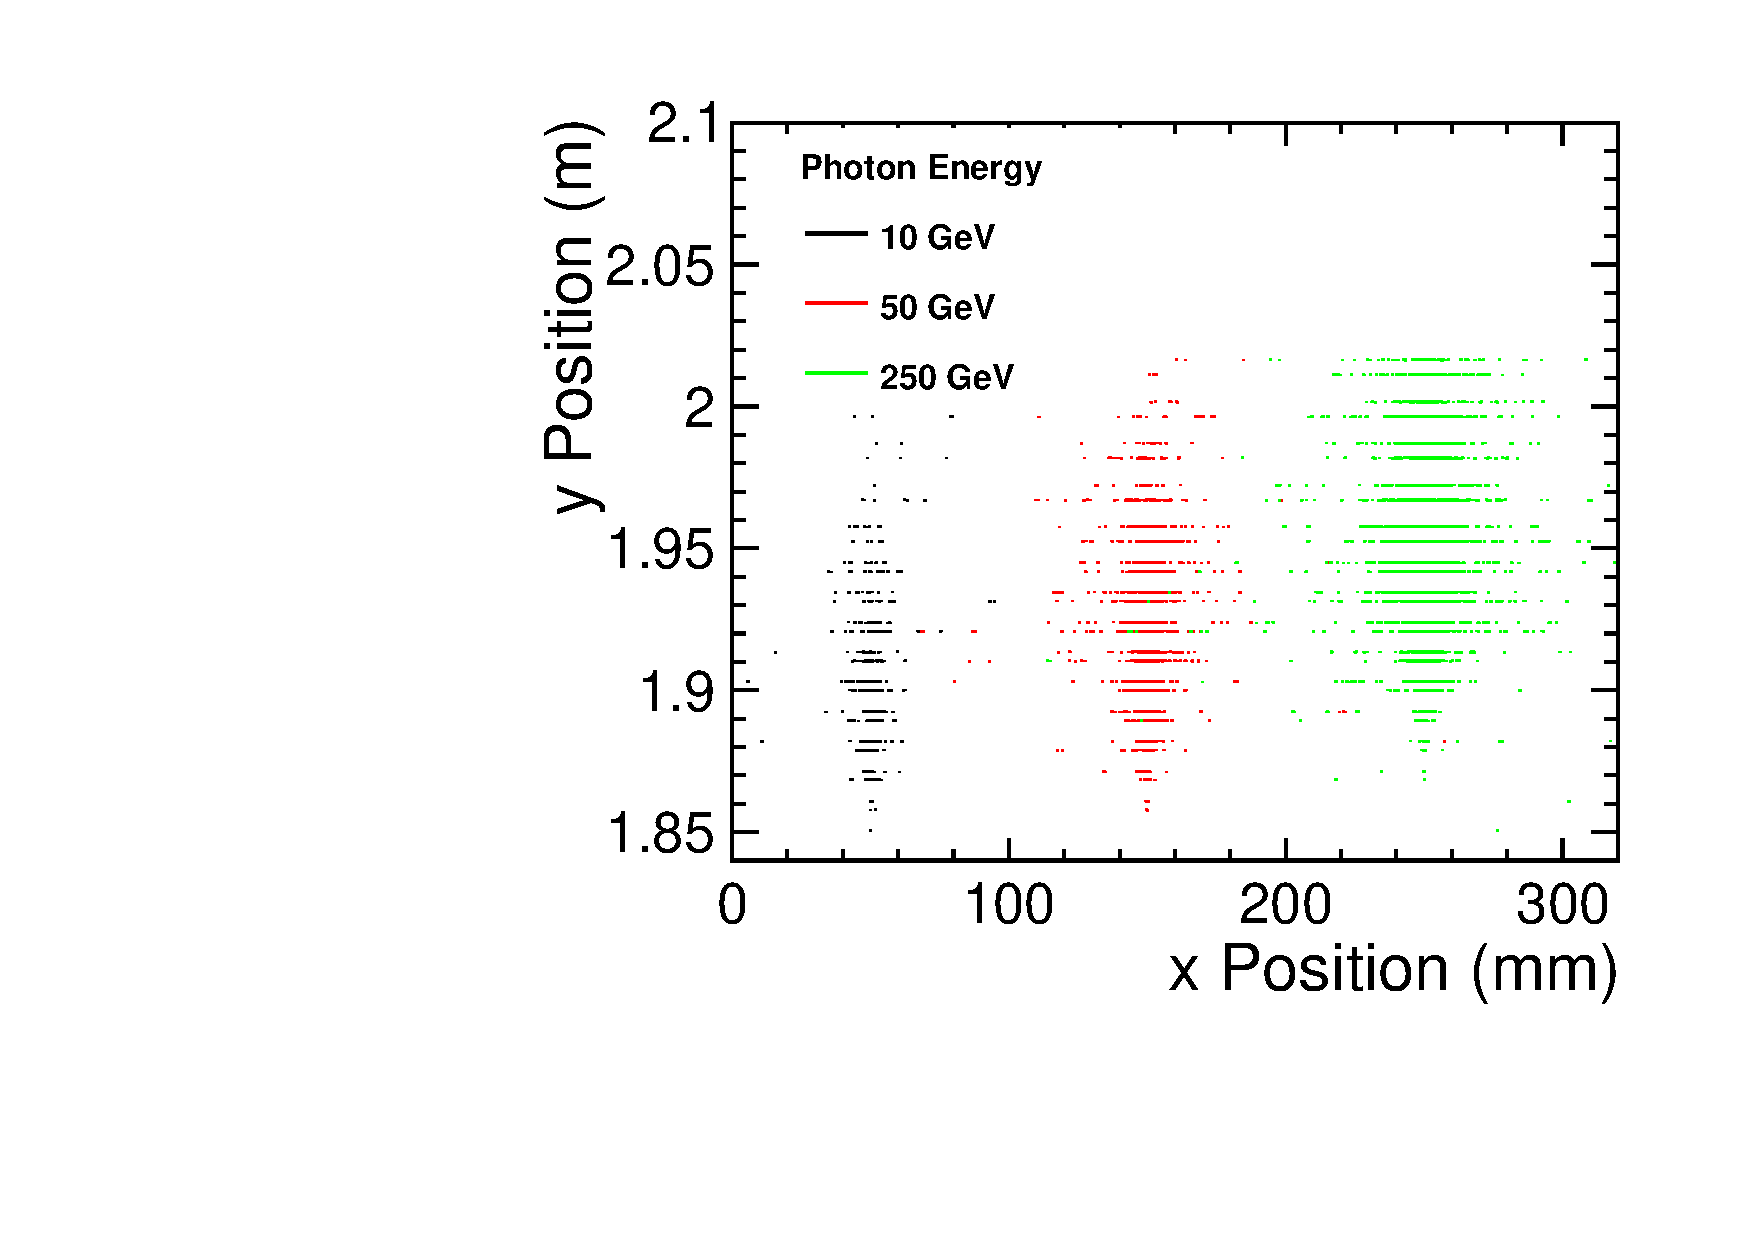
\includegraphics[width=0.7\textwidth,keepaspectratio]{DECALStudies/fig/ExampleEvents}
  \caption[Example of how EM showers look in a \ac{DECAL} with 10$\times$10~$\mu$m$^2$ pixels for various photon energies.]{Example of how EM showers look in a \ac{DECAL} with 10$\times$10~$\mu$m$^2$ pixels for various photon energies. The y coordinate here represents the radial distance from the centre of the full detector.}
  \label{fig:exampleevents}
\end{figure}

Once the geometry was implemented, events were generated using the built in Mokka particle gun to fire photons through the \ac{ECAL}. When doing this the gun was placed perpendicular to the \ac{ECAL} surface and immediately in front of the \ac{ECAL} to prevent showers forming earlier in the detector from interactions with the inner components such as the tracker. Photon were produced in 10 GeV intervals between 10 GeV and 100 GeV. For each energy, 10,000 events were generated to produce a large enough statistical sample to work with. Events were then generated using five different epitaxial thicknesses between 12 and 20 $\mu$m. Additional samples were generated at 250 GeV representing the maximum energy possible at \ac{ILC}. In this case only 5000 events were generated per epitaxial layer due to the considerably longer simulation times. In total this corresponds to a total of $\sim$ 500,000 events generated. An example of what these events look like in the detector is shown in \reffig{fig:exampleevents}.

In order to be realistic, thresholds were applied on the energy deposited in a pixel as in practice this is always necessary to remove hits coming from electrical/thermal noise. The amount of energy deposited by a particle in a thin layer of material will typically follow a landau distribution. The threshold was chosen to be half of the most probable value (MPV) of the landau distribution to provide a balance between the amount of signal loss and potential background acceptance. The value of the MPV was found by fitting the energy ditributions measured in the simulation. For doing this, 10 GeV photons and 100$\times$100 $\mu$m$^2$ pitch pixels were used to prevent influence from saturation or from boundary effects where a particle deposits low amounts of energy from crossing the boundary between two pixels within one layer. As the amount of energy depsosited depends only on the epitaxial layer thickness and not the pixel pitch, the thresholds were only evaluated once for each epitaxial thickness then applied uniformly across all pitches. An example of one of the fits used in determining the threshold is shown in \reffig{fig:thresholdfit}.

\begin{figure}
  \centering
  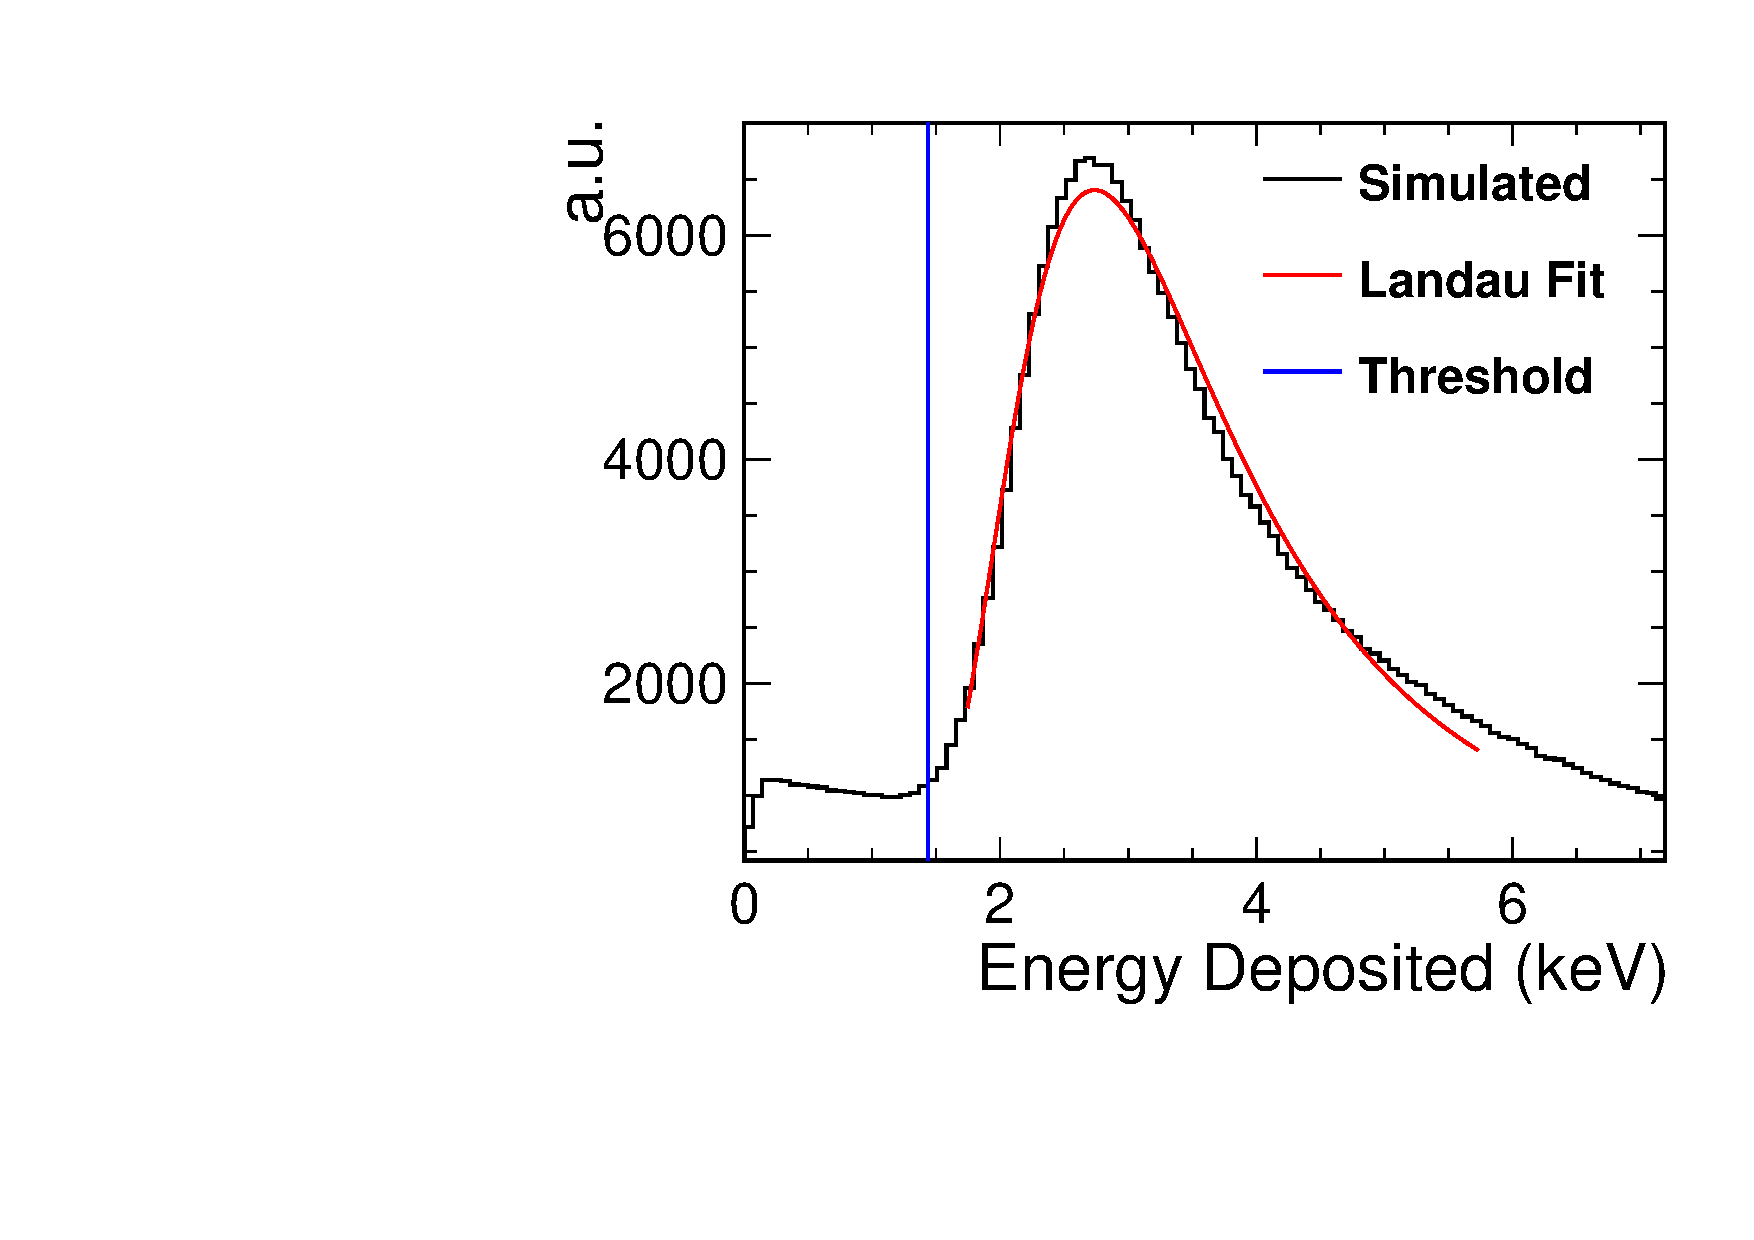
\includegraphics[width=0.7\textwidth,keepaspectratio]{DECALStudies/fig/Landau_100x12_10GeV.pdf}
  \caption{Energy deposited in a 100$\times$100 $\mu$m$^2$ pitch, 12$\mu$m thick pixel by a 10 GeV photon. The landau fit and resulting choice of threshold are also shown.}
  \label{fig:thresholdfit}
\end{figure}


\section{Pixel Design Optimization}

Ultimately the performance of any calorimeter is measured by the energy resolution, $\sigma_E/E$ , it can achieve. As such it is important to explain how this is defined for a digital calorimeter. Naively one could work on the basis that the energy of a particle is proportional to the number of particles produced in a shower and so define the resolution to be $\sigma_N/N$ where $N$ is the number of hits in the detector. While this is theoretically true, it fails to account for the fact the number of particles produced in the shower may not be proportional to the number of hits measured due to effects such as multiple occupancies. A more reliable definition of the resolution has been found to come from first creating a calibration curve defining the relationship between the true energy of a particle, then using this curve to map back from the number of particles to a reconstructed energy for a particle. The energy resolution is then calculated by performing a gaussian fit to the reconstructed particle energies and defining the resolution to be $\sigma_{E,Gaus}/E$. In the case of a perfect detector, this resolution should be equivalent to $\sigma_N/N$ as $N$ is linearly proportional to $E$. In all cases, the calibration curves are produced using one fifth of the statistical sample and the remaining four fifths are used to evaulate the energy resolution. Examples of how these calibration curves look for different pixel configurations are shown in \reffig{fig:calibrationcurves}. For wider pixels it is observed that the energy to hits relationship becomes non linear indicating detector saturation is occuring. 

\begin{figure}
  \centering
  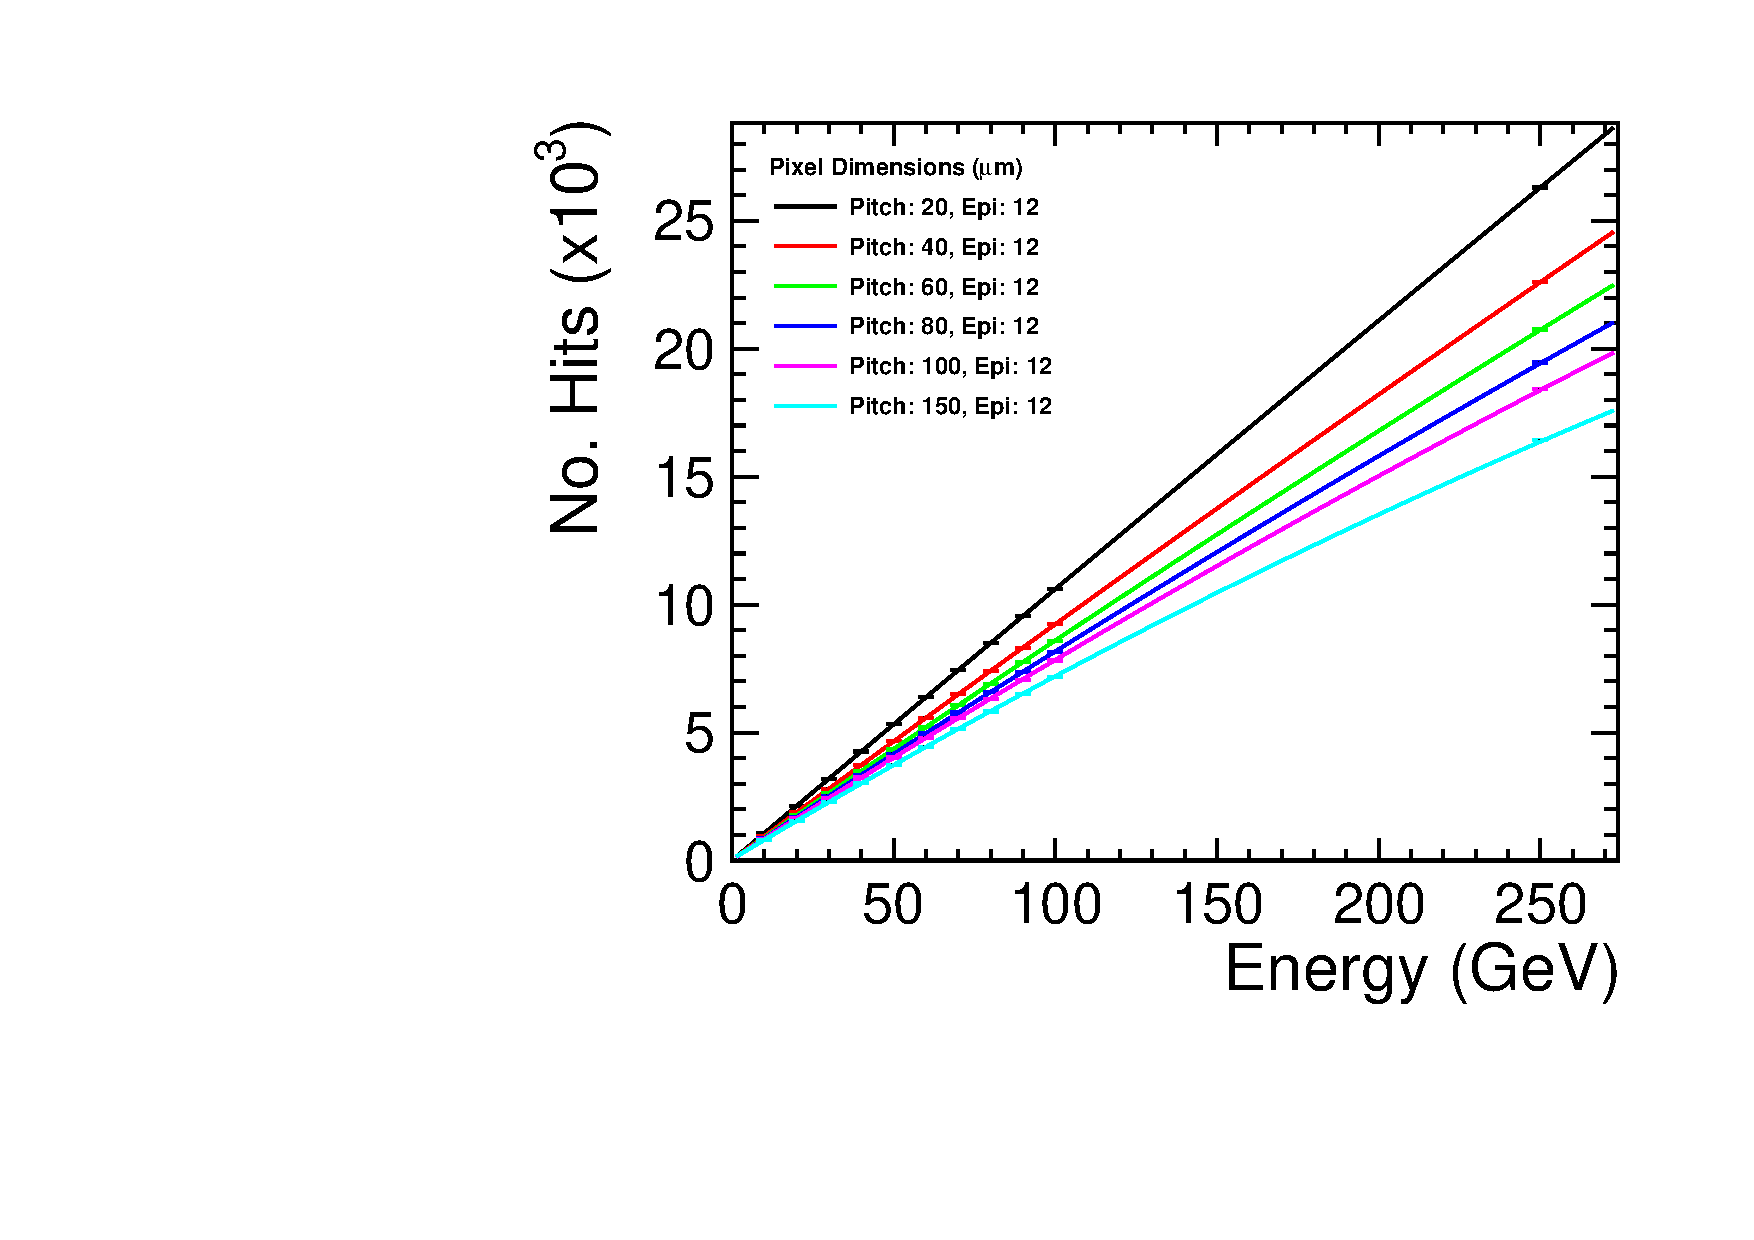
\includegraphics[width=0.7\textwidth,keepaspectratio]{DECALStudies/fig/CalibrationCurves.pdf}
  \caption{Calibration curves describing the relationship between the number of pixel hits observed and the energy of the incident particle for various pixel configurations.}
  \label{fig:calibrationcurves}
\end{figure}

\begin{figure}
  \centering
  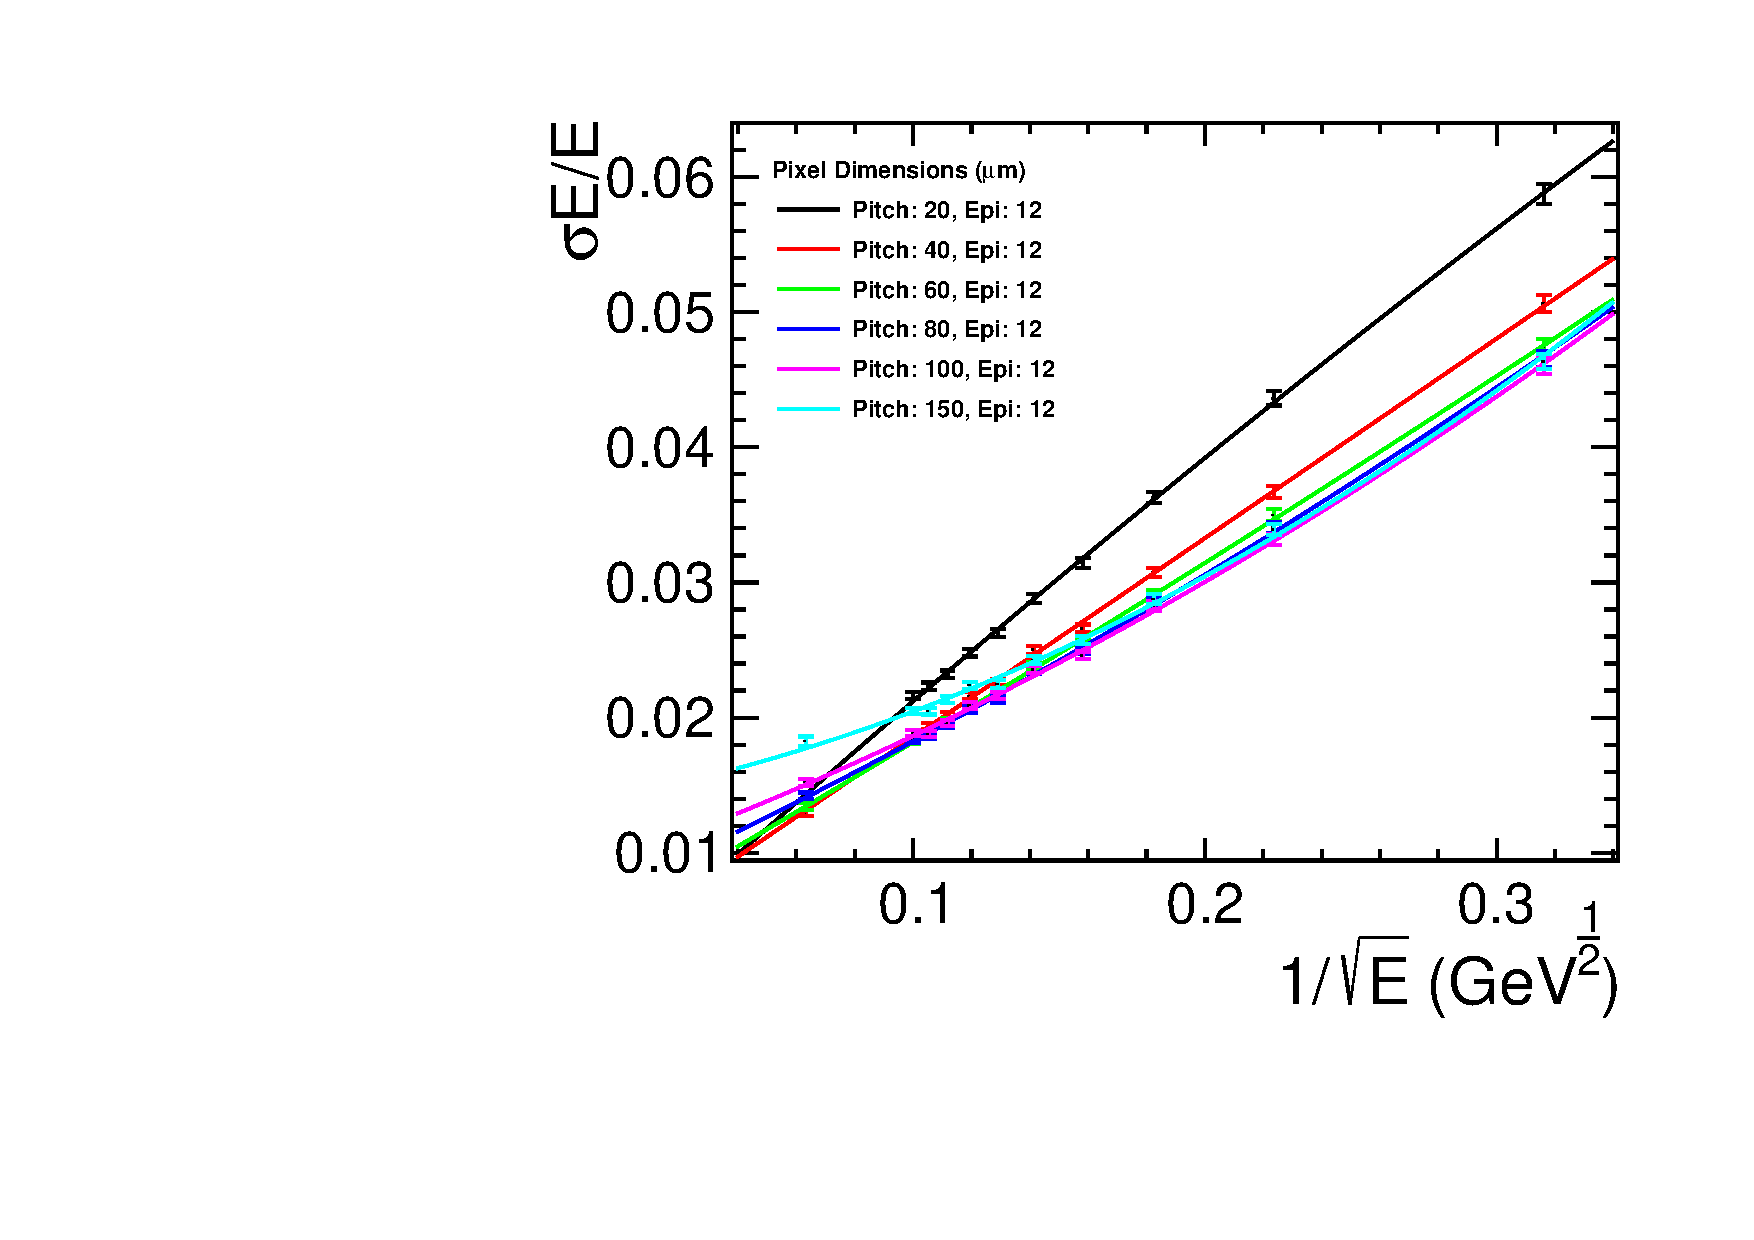
\includegraphics[width=0.7\textwidth,keepaspectratio]{DECALStudies/fig/ResolutionFits.pdf}
  \caption{Energy resolution curves describing the variation of the energy resolution with the energy scale}
  \label{fig:resolutionfits}
\end{figure}

Having generated the calibration curves, the energy resolution was then determined for every photon energy and pixel configuration. The performance for each pixel configuration is evaluated by performing a second order polynomial fit to $\sigma_E/E$ vs 1/$\sqrt{E}$ (see \reffig{fig:resolutionfits}). This method allows the parameters a, b and c to be extracted in accordance with \refeq{eq:resolutionformula}, where a is the stochastic term, b is the noise term and c is the constant/leakage term. Typically the resolution of an \ac{ECAL} can be expected to be dominated by the stochastic term. 

\begin{equation}
  \label{eq:resolutionformula}
  \frac{\sigma_E}{E}=\frac{a}{\sqrt{E}} \oplus \frac{b}{E} \oplus c
\end{equation}

The values of a, b and c for every pixel configuration are shown in \reffigs{fig:stochasticterm}, \ref{fig:noiseterm} and \ref{fig:constantterm}. One can see that the stochastic and noise terms dominate the overall resolution, however they show very different dependencies on the pixel configuration. The stochastic is seen to be lowest for wider pixel pitches whereas the noise term is lowest for the narrower pitches. One can trivially explain the distribution in the noise term as arising from saturation effects as for wider pixels the granularity of the detector will be less than the density of the EM showers. This results in a non linear response for the detector which gets translated into a non linear energy resolution and so a large second order term in the 1/$\sqrt{E}$ fit. Further evidence for this explanation can be seen in \reffig{fig:occupancy} which shows the occupancy per pixel for 100 GeV events increases with pixel pitch. This effect is also easily seen in \reffig{fig:resolutionfits} where for the wider pixels the performance is reasonably consistent for lower energies but diverges at the highest energies where saturation begins to occur making the resolution worse and introducing a second order term to the distribution.

\begin{figure}
  \centering
  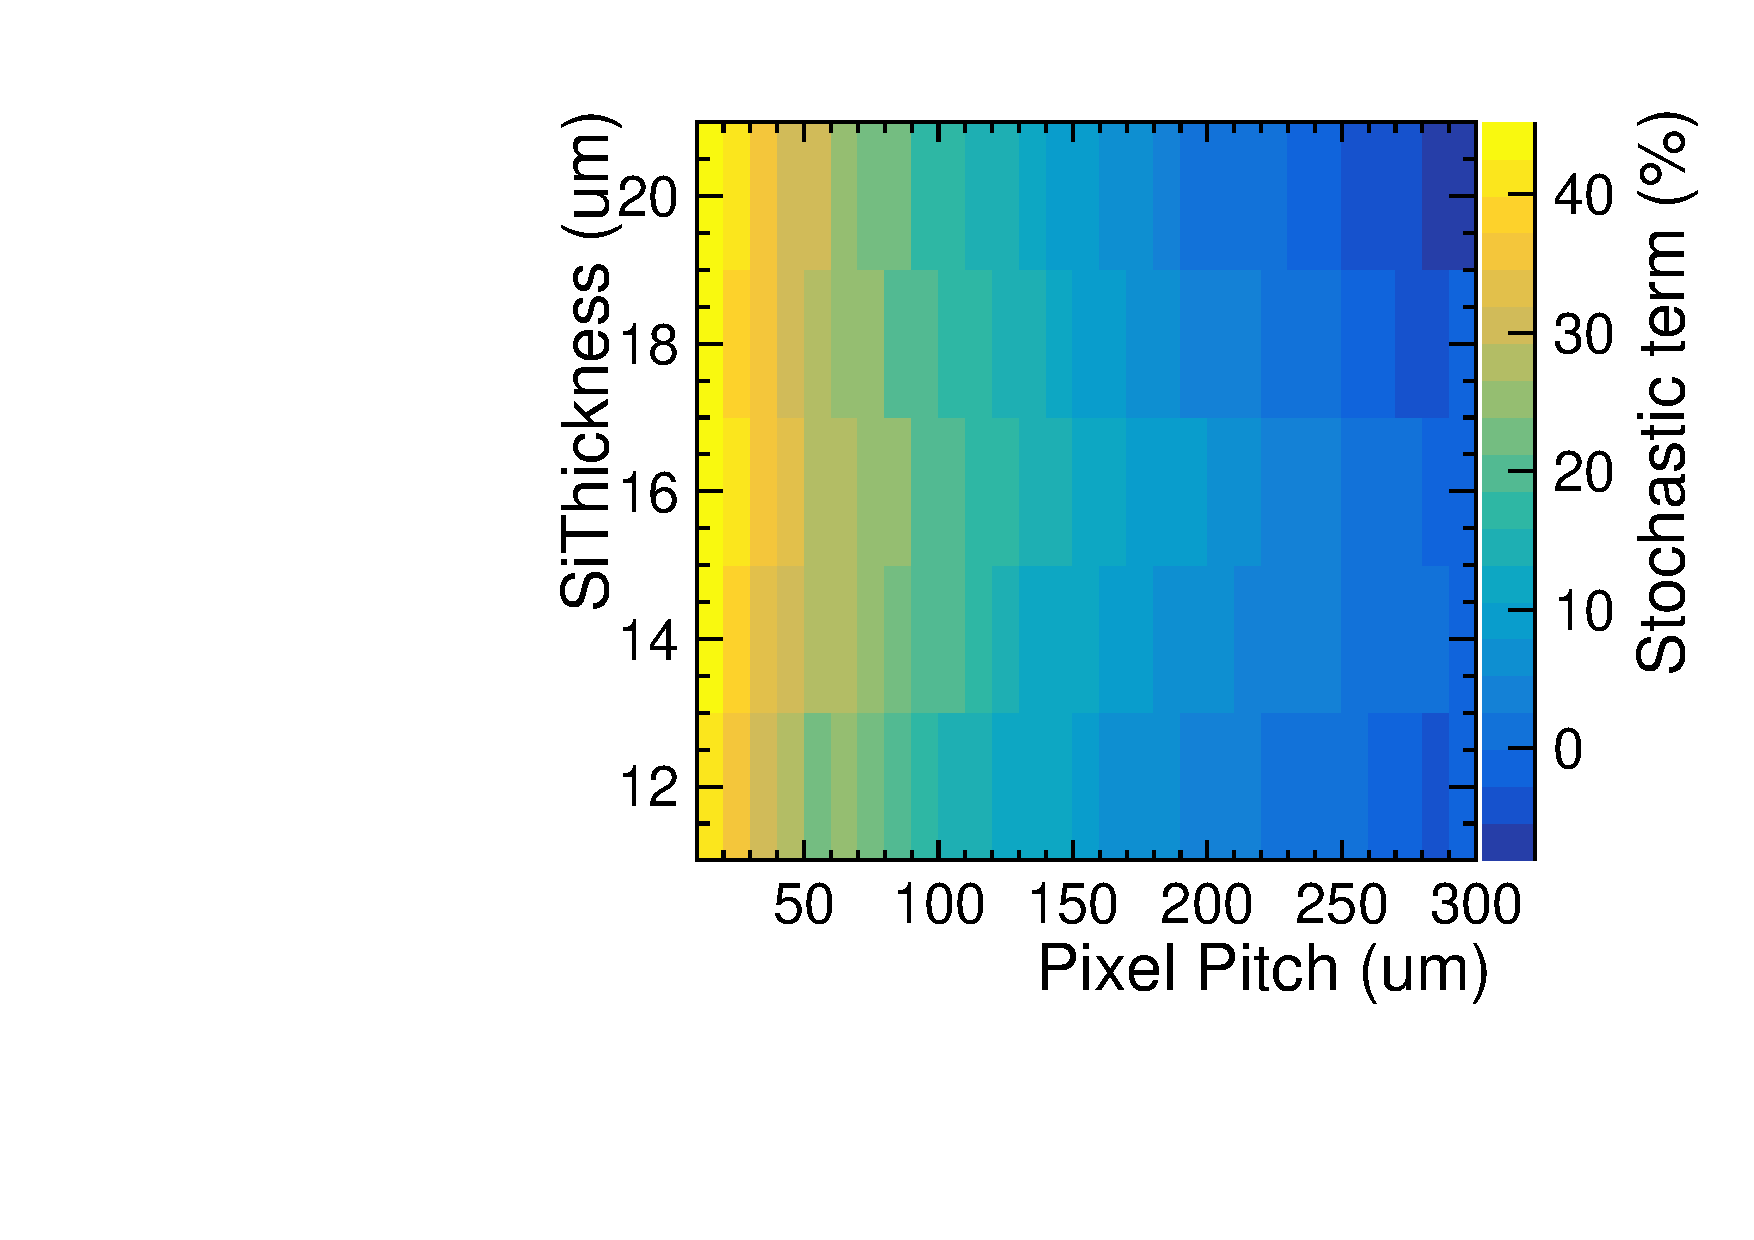
\includegraphics[width=0.7\textwidth,keepaspectratio]{DECALStudies/fig/2DRawStochastic.pdf}
  \caption{Stochastic term of the energy resolution fits for all pixel configurations}
  \label{fig:stochasticterm}
\end{figure}
\begin{figure}
  \centering
  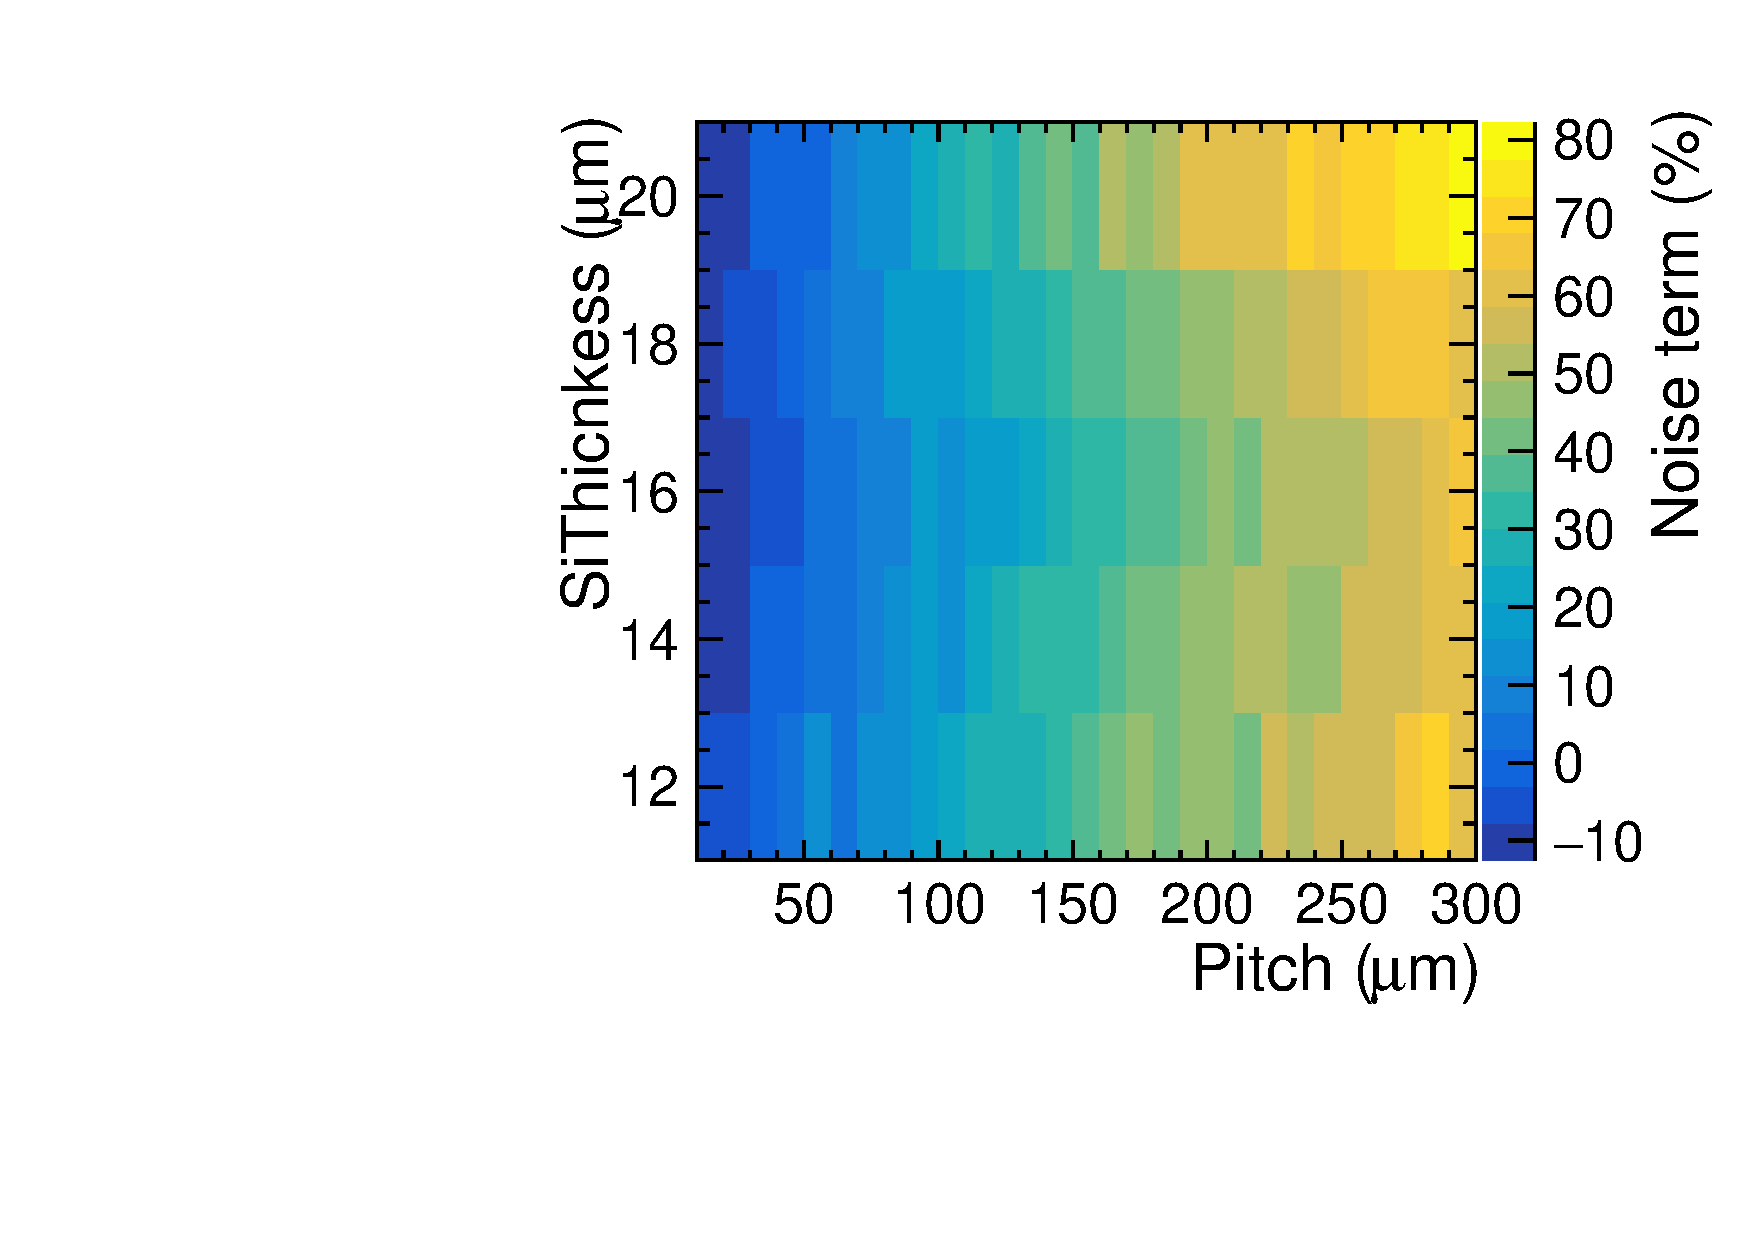
\includegraphics[width=0.7\textwidth,keepaspectratio]{DECALStudies/fig/2DRawNoise.pdf}
  \caption{Noise term of the energy resolution fits for all pixel configurations}
  \label{fig:noiseterm}
\end{figure}
\begin{figure}
  \centering
  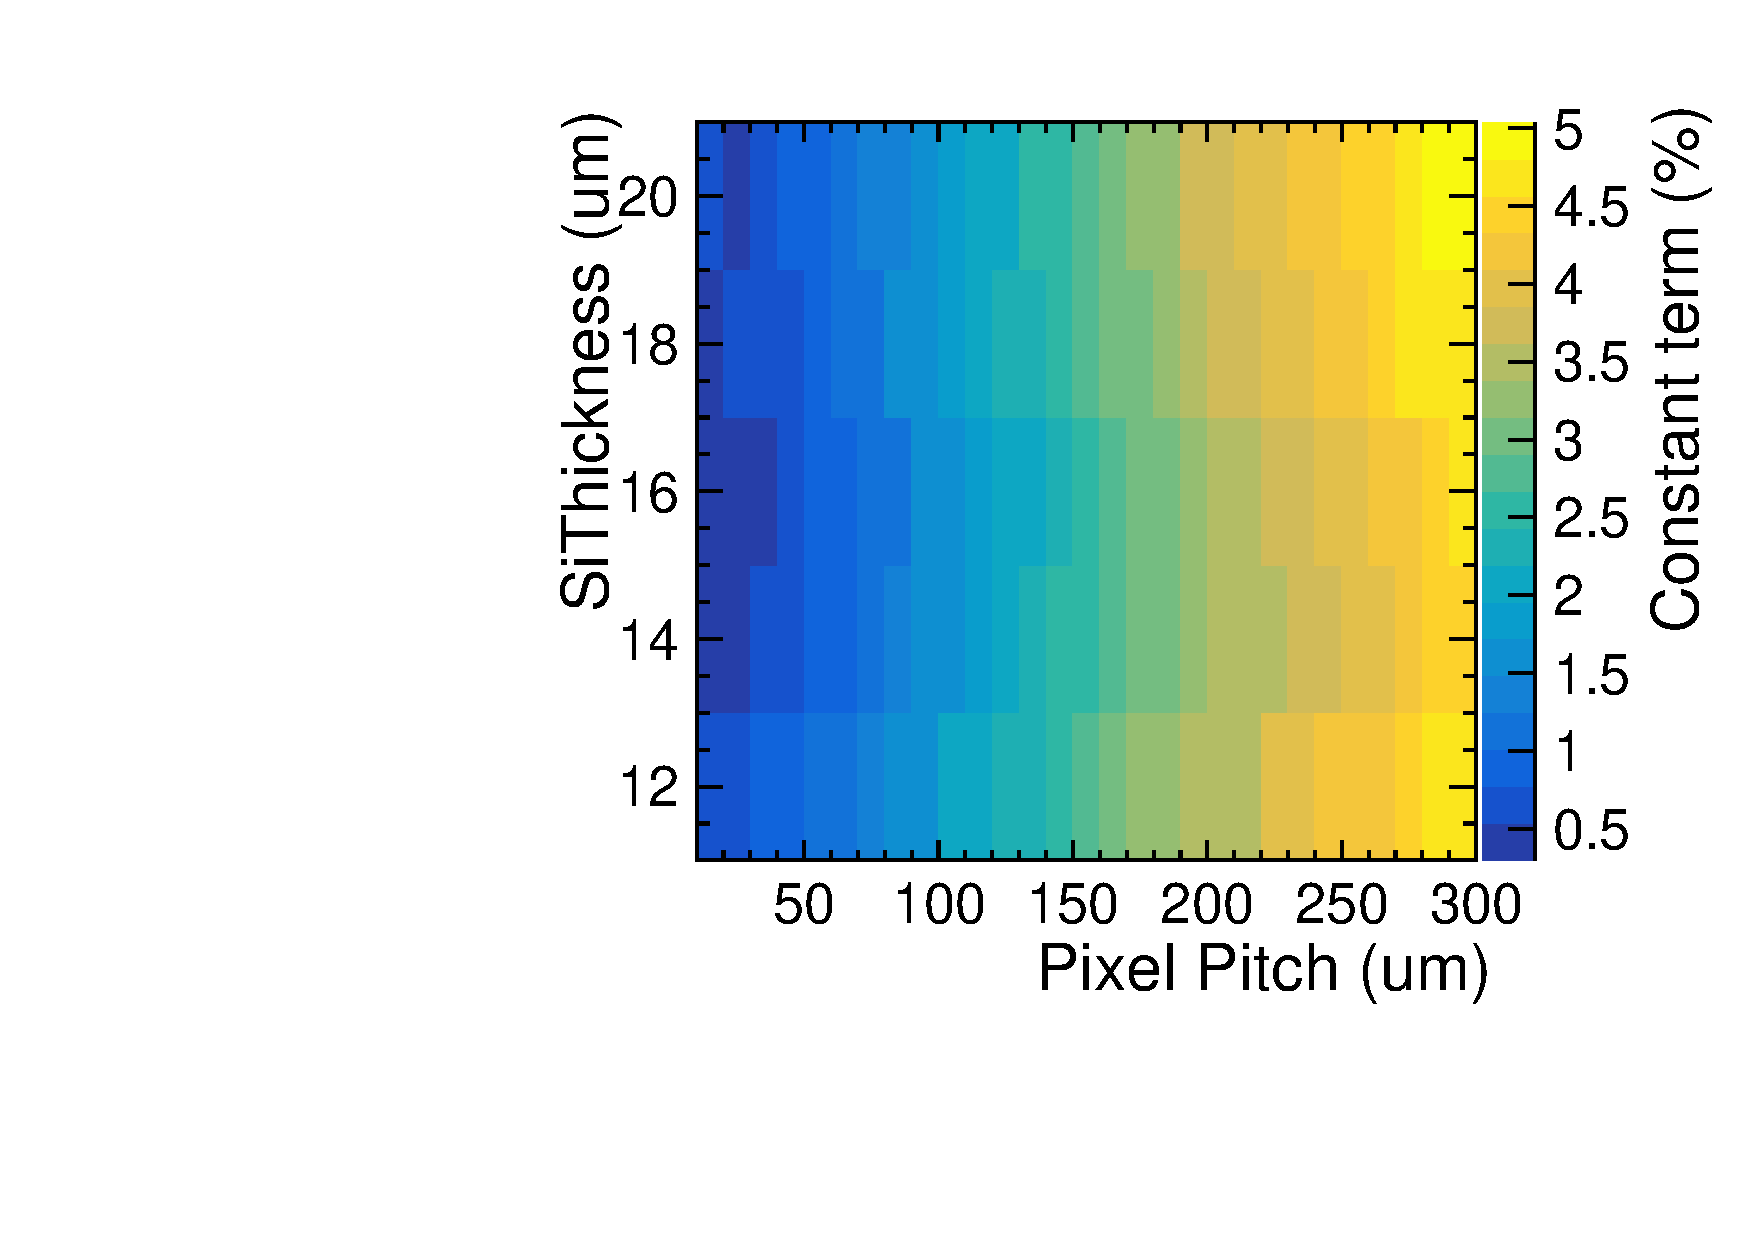
\includegraphics[width=0.7\textwidth,keepaspectratio]{DECALStudies/fig/2DRawConstant.pdf}
  \caption{Constant term of the energy resolution fits for all pixel configurations}
  \label{fig:constantterm}
\end{figure}

\begin{figure}
  \centering
  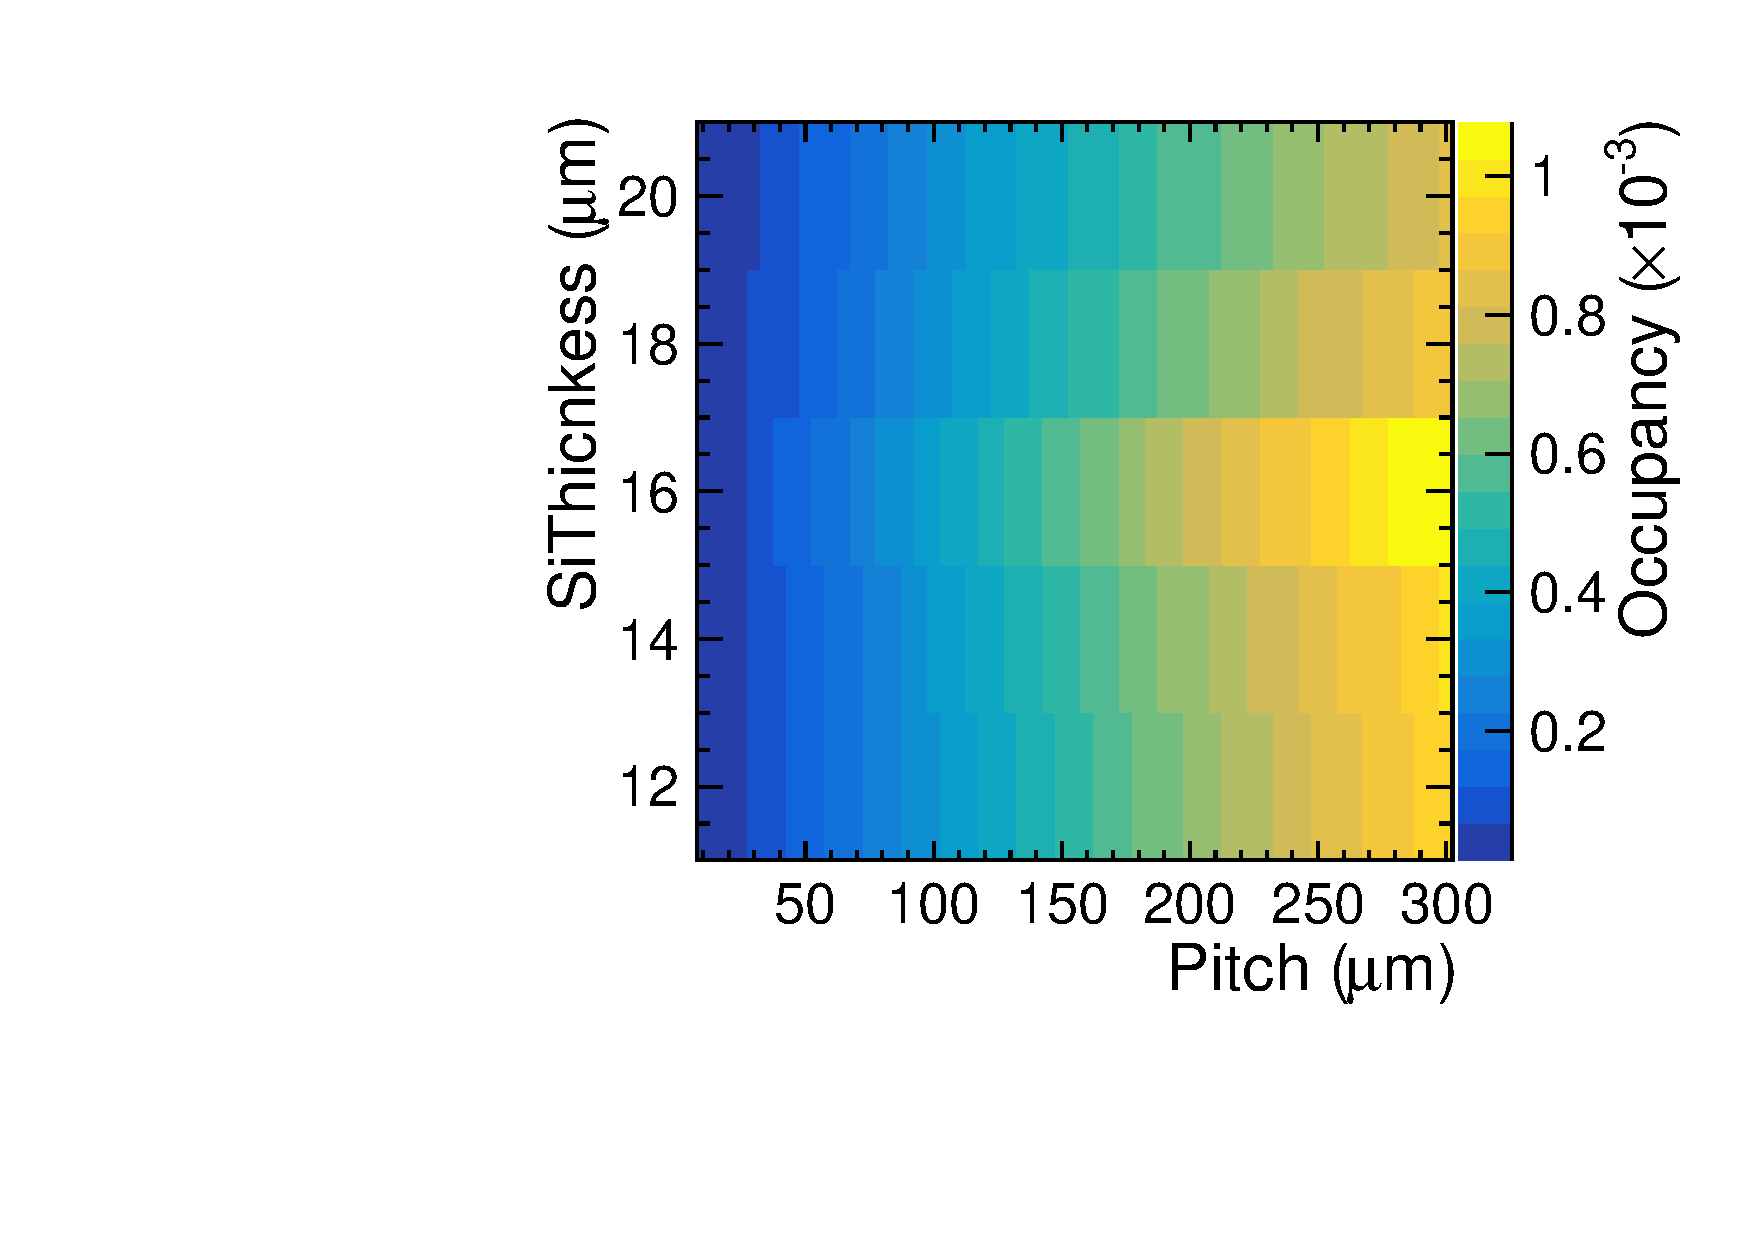
\includegraphics[width=0.7\textwidth,keepaspectratio]{DECALStudies/fig/Occupancy_100GeV.pdf}
  \caption{Pixel occupancy for 100 GeV photons.}
  \label{fig:occupancy}
\end{figure}


To understand the stochastic term requires examination of the landau distributions as shown in \reffigs{fig:landaupitches} and \ref{fig:landauthickness}. One can see that as the aspect ratio decreases, a secondary peak appears in the energy deposition distribution at low energies. This is a result of particles crossing between pixels and so leaving only a fraction of the expected energy per layer in each pixel. The result of the boundary crossings is that there is a greater fluctuation on the number of pixels above threshold as rather than consistently observing one hit per particle per layer, it is possible to also get no hits if the deposits across both pixels are below threshold, or more likely an additional hit from both deposits being above threshold. 

\begin{figure}
  \centering
  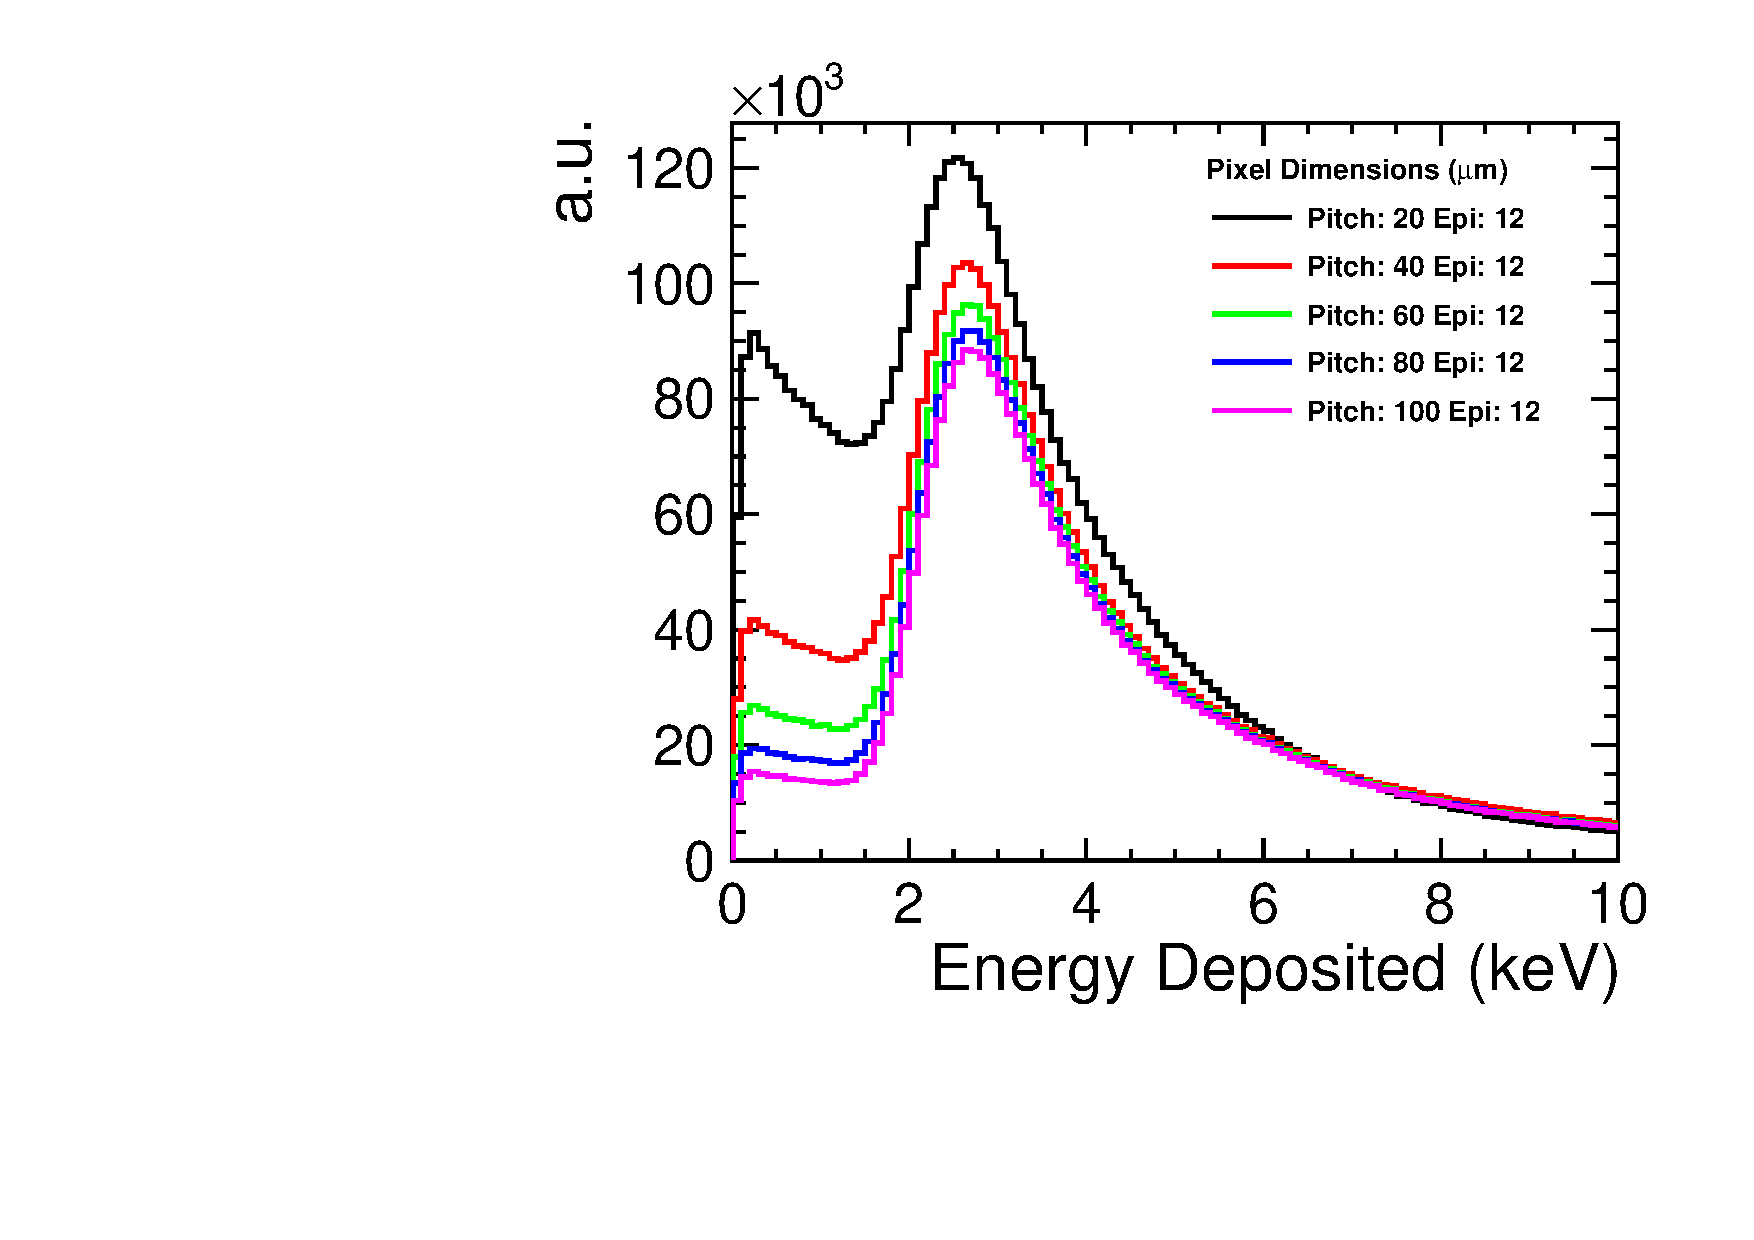
\includegraphics[width=0.7\textwidth,keepaspectratio]{DECALStudies/fig/LandauVsPitch.pdf}
  \caption{Variation in the landau distributions for 10 GeV photons as a function of the pixel pitch. All distributions normalised to unity.}
  \label{fig:landaupitches}
\end{figure}
\begin{figure}
  \centering
  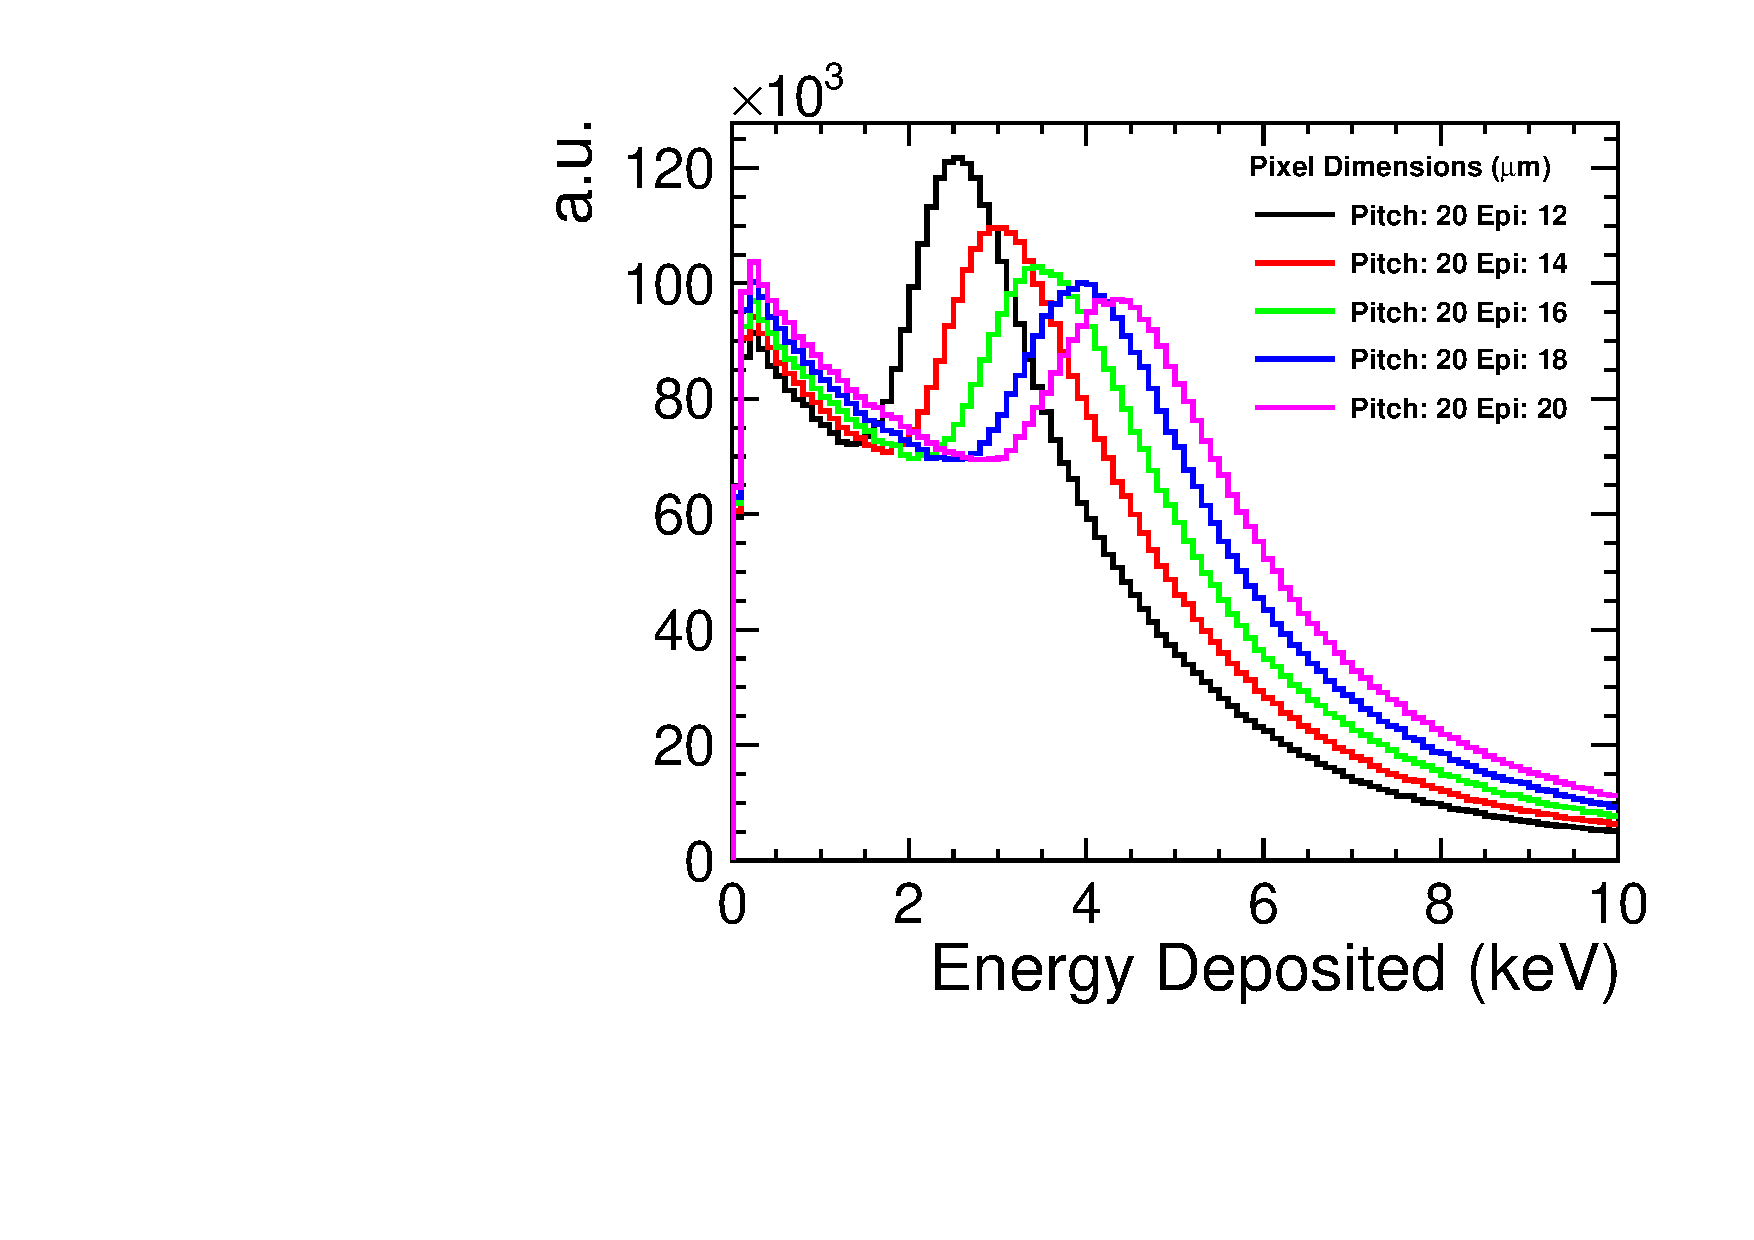
\includegraphics[width=0.7\textwidth,keepaspectratio]{DECALStudies/fig/LandauVsEpi.pdf}
  \caption{Variation in the landau distributions for 10 GeV photons as a function of the epitaxial thickness. All distributions normalised to unity.}
  \label{fig:landauthickness}
\end{figure}

The optimal pixel configuration should provide a balance between the boundary crossing and multiple occupancy effects. Because the saturation level is a function of the incident particle energy, the optimal design will vary depending on the energy scale the detector is intended to be used at. For lower energy scales a wider pixel is optimal as the saturation is inherently low due to the low shower density and the wide pitch will then minimise boundary crossings. For higher energies the saturation rate will dominate and so a narrower pixel is preferred. In both cases a thinner pixel is preferred to minimise boundary crossings. The net resolutions observed at three different energy scales are shown in \reffigs{fig:resolution10}, \ref{fig:resolution50} and \ref{fig:resolution250}. The variation in the optimal configuration is seen to agree with that predicted from the above boundary crossing and occupancy considerations.

\begin{figure}
  \centering
  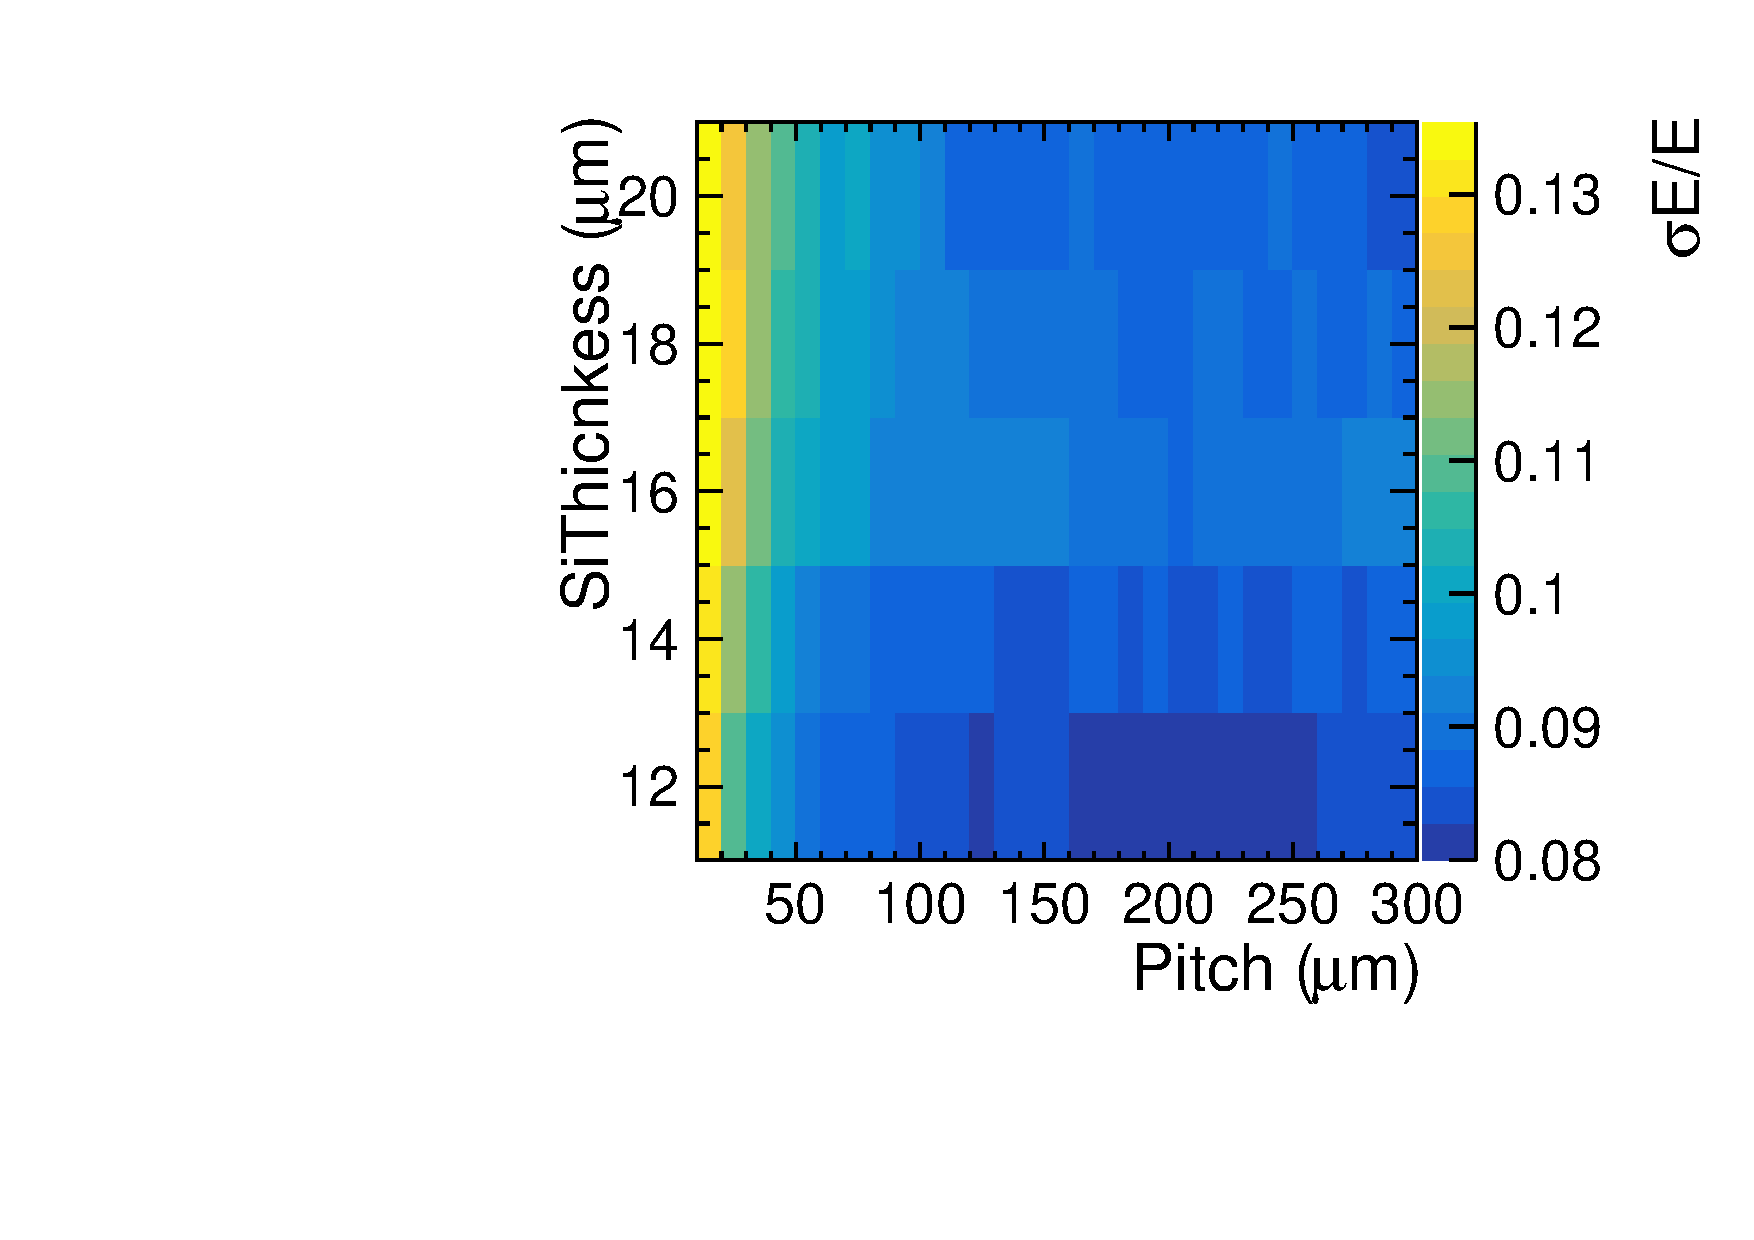
\includegraphics[width=0.7\textwidth,keepaspectratio]{DECALStudies/fig/2DRawRes10.pdf}
  \caption{Energy resolution for 10 GeV photons.}
  \label{fig:resolution10}
\end{figure}

\begin{figure}
  \centering
  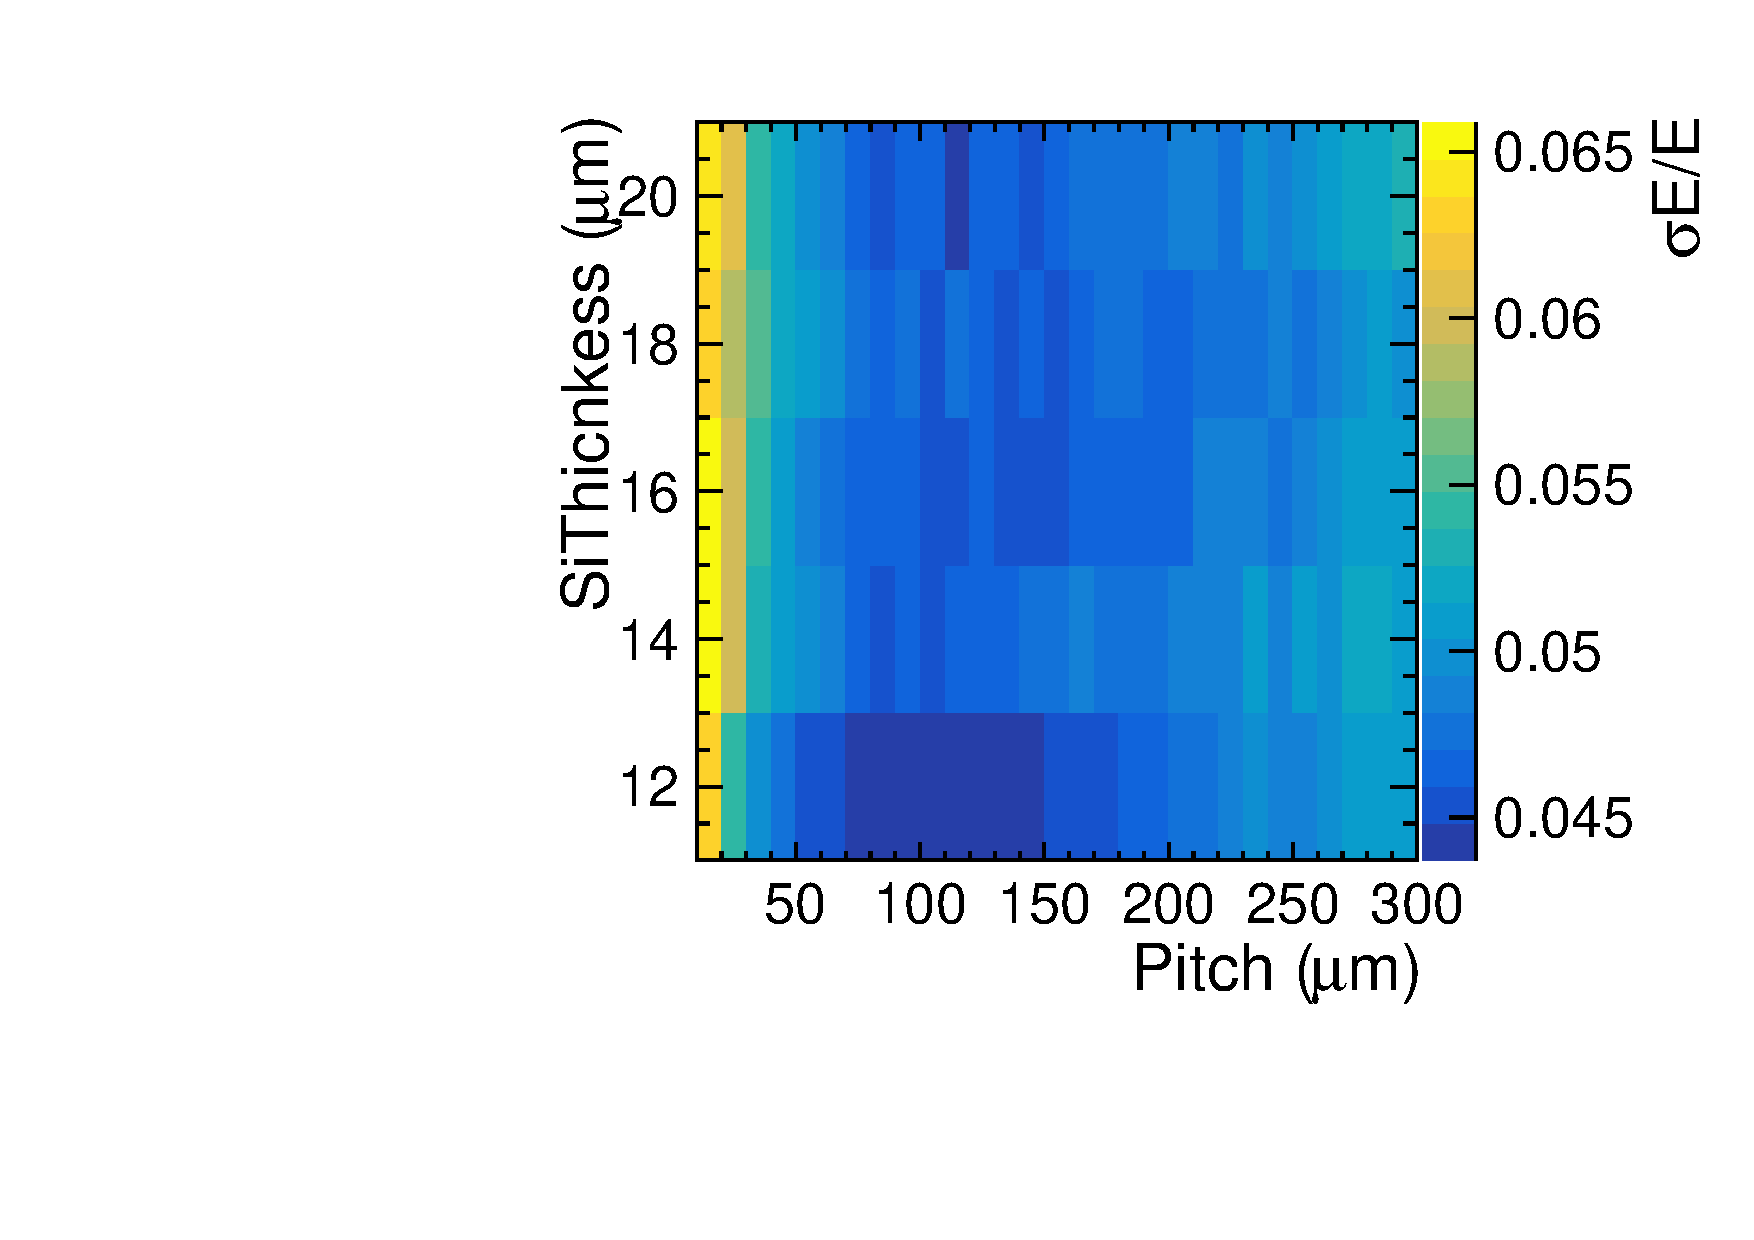
\includegraphics[width=0.7\textwidth,keepaspectratio]{DECALStudies/fig/2DRawRes50.pdf}
  \caption{Energy resolution for 50 GeV photons.}
  \label{fig:resolution50}
\end{figure}

\begin{figure}
  \centering
  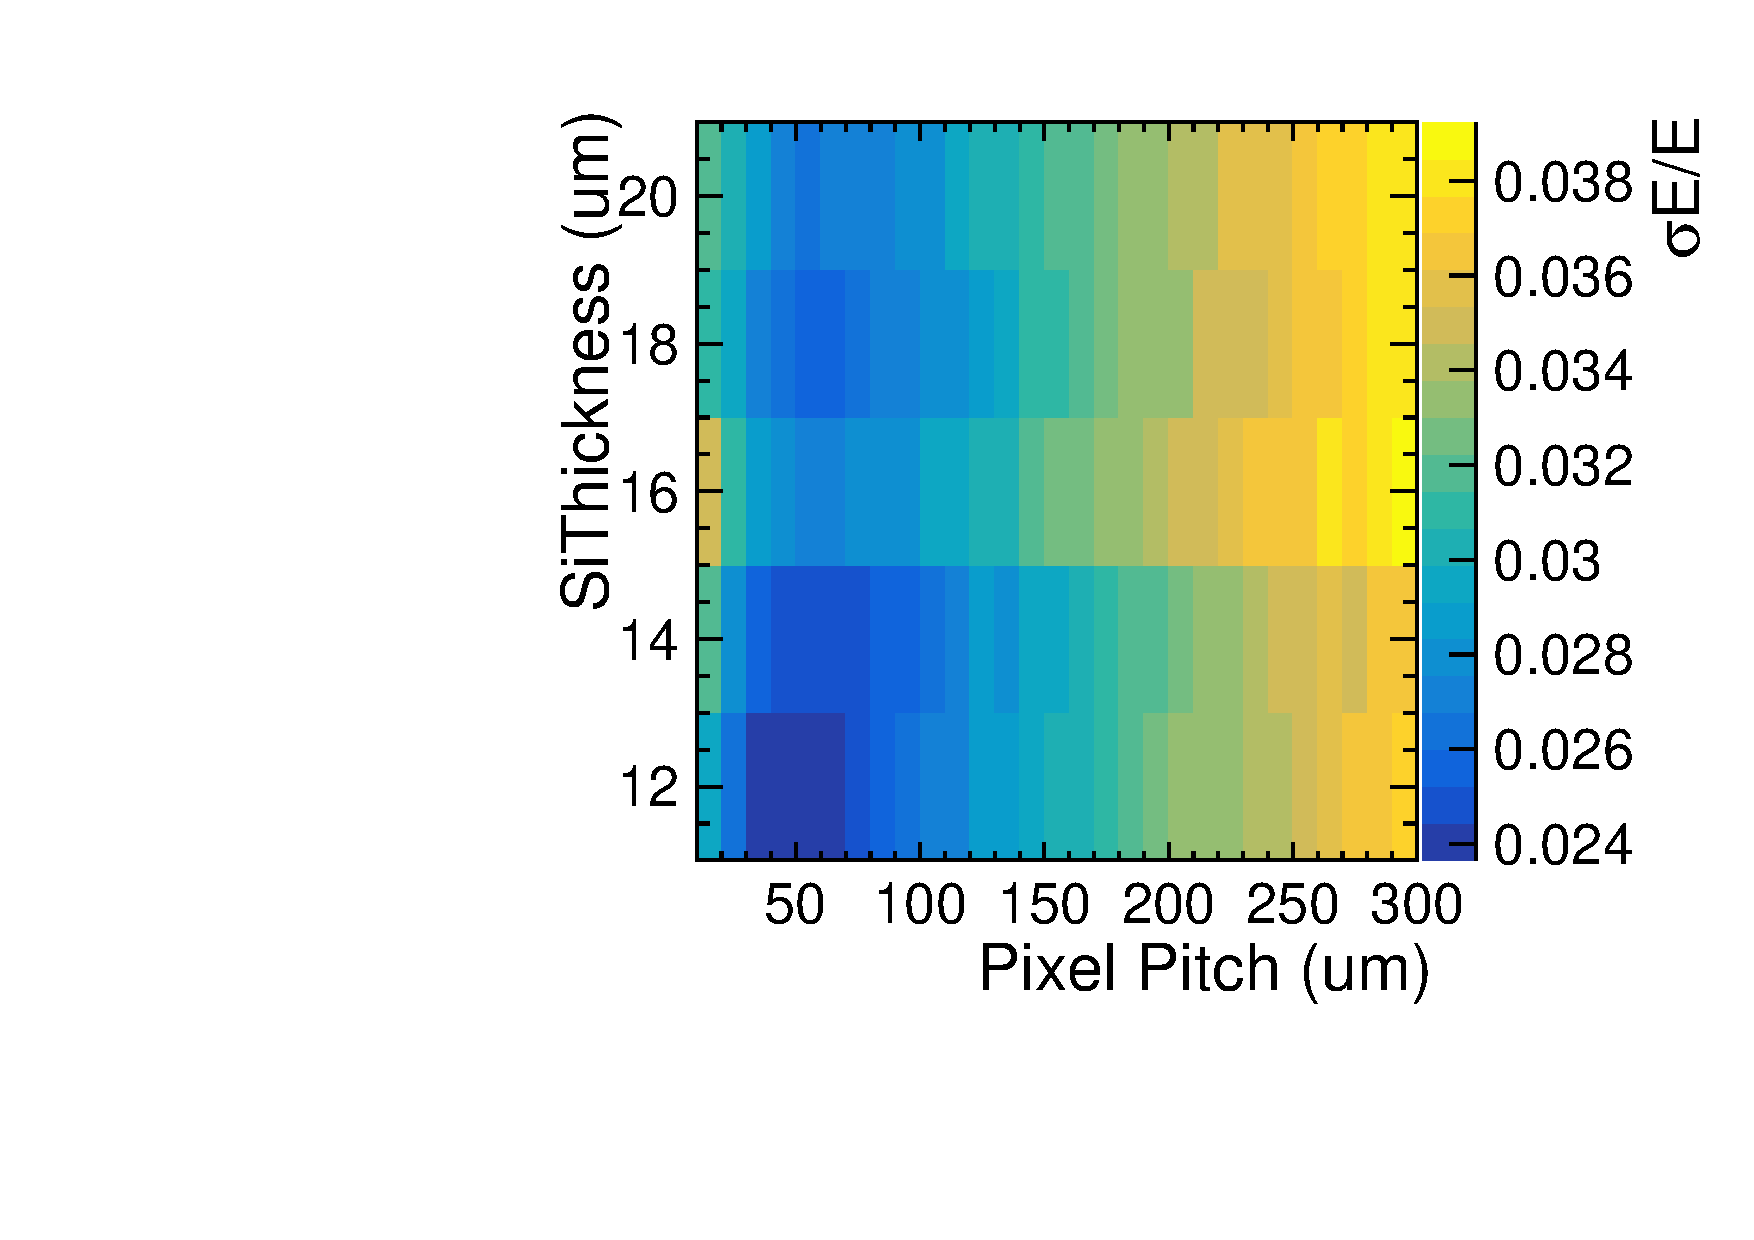
\includegraphics[width=0.7\textwidth,keepaspectratio]{DECALStudies/fig/2DRawRes250.pdf}
  \caption{Energy resolution for 250 GeV photons.}
  \label{fig:resolution250}
\end{figure}

\section{DigiMAPs}

While the above simulations highlight the dominant effects that must be considered in designing a digital calorimeter, they remain somewhat unrealistic. In particular they lack effects such as charge collection efficiencies within the pixels, thermal/electronic noise and the effects of clustering. These effects are not possible to study within standard GEANT4 simulations, instead they are added in later using a package referred to as DigiMAPS developed by the \ac{CALICE} collaboration. This package takes the output hits from MOKKA, applies the effects of added levels of realism to remove/create new hits, then outputs an updated collection of hits for analysis. The effects that have been considered are listed below.

\begin{itemize}
\item Charge spread: When a particle deposits energy within a pixel it does so by producing electron hole pairs within the material which are then collected by diodes. In practice, there will be a finite efficiency for collecting the deposited charge which will depend on how the collection diodes are placed throughout the pixel and where the particle enters the pixel. Modelling of the charge collection requires detailed TCAD simulations performed using external software. Within DigiMAPS, the modelling of this is provided for only one pixel configuration corresponding to a pixel with 50~$\mu$m pitch, 18~$\mu$m epitaxial thickness and four charge collection diodes arranged in a square. DigiMAPS used the efficiency map for this configuration to apply an efficiency scaling on the energy deposited by a particle based on where within the pixel it enters. Unfortunately the software required to create the efficiency maps is not readily available and so it was not possible to examine how the charge efficiency impacts any other pixel configuration.
  
\item Noise Effects: It is possible for noise to be produced either from thermal fluctuations within the silicon or from the electronics associated with the diode and readout systems. For \ac{DECAL} applications it is expected that the noise will follow a poisson distribution with a mean of 30 electron hole pairs per pixel. This noise is typically problematic as it can result in fake hits being produced in pixels with no signal contribution leading to overcounting of hits, however it can also be beneficial in the case of genuine hits where it can push hits with low energy deposits above the threshold preventing them from being missed. As such, in later plots the noise contributions will be split into the cases where noise is only added to pixels containing signal deposits and when it is added to all pixels throughout the detector.
  
\item Dead space: In order to accomodate the necessary electronics required for each pixel, there will typically be a certain amount of dead space per pixel which will be insensitive to any particles hitting it. Within DigiMAPS this is accounted for by ignoring hits within the first 10\% of the width of each pixel.
  
\item Threshold spread: Due to imperfections in the pixel manufacturing process, pixels will typically show a non uniform response to incoming particles. This effect is normally minimsed via a calibration procedure known as trimming which effectively corresponds to measuring the response of each pixel and setting the thresholds accordingly to get a uniform response. For the level of logic available within proposed \ac{DECAL} designs it is expected that this procedure will leave only a 1\% non uniformity in the pixel response. This is accounted for within DigiMAPS by applying a gaussian spread to the threshold of each pixel with a width of 1\%.
  
\item Clustering: In any realistic experiment, the energy resolution of a calorimter will not be taken to be the sum of all energy depsoited within the calorimeter, instead some level of pattern recognition will be done to remove noise events and group signal hits to reduce the volume of data being read from the detector. This process is referred to as clustering. Here we use a very simplistic clustering method to illustrate the benefits it can have. For each hit the number of immediately adjacent hits are counted. If all 8 adjacent pixels contain hits, the pixel is deemed a cluster and the neighbouring hits are discarded. If no adjacent pixels are hit then the pixel will simply be declared a cluster by itself. If 1-7 of the adjacent pixels have hits, each neighbour is examined and assigned a score corresponding to the number of its neighbours that contain hits. The scores of the original hit and all it's neighbours are compared and the pixel with the highest score is declared to be a cluster and it's neighbours are removed.  
\end{itemize}

\begin{figure}
  \centering
  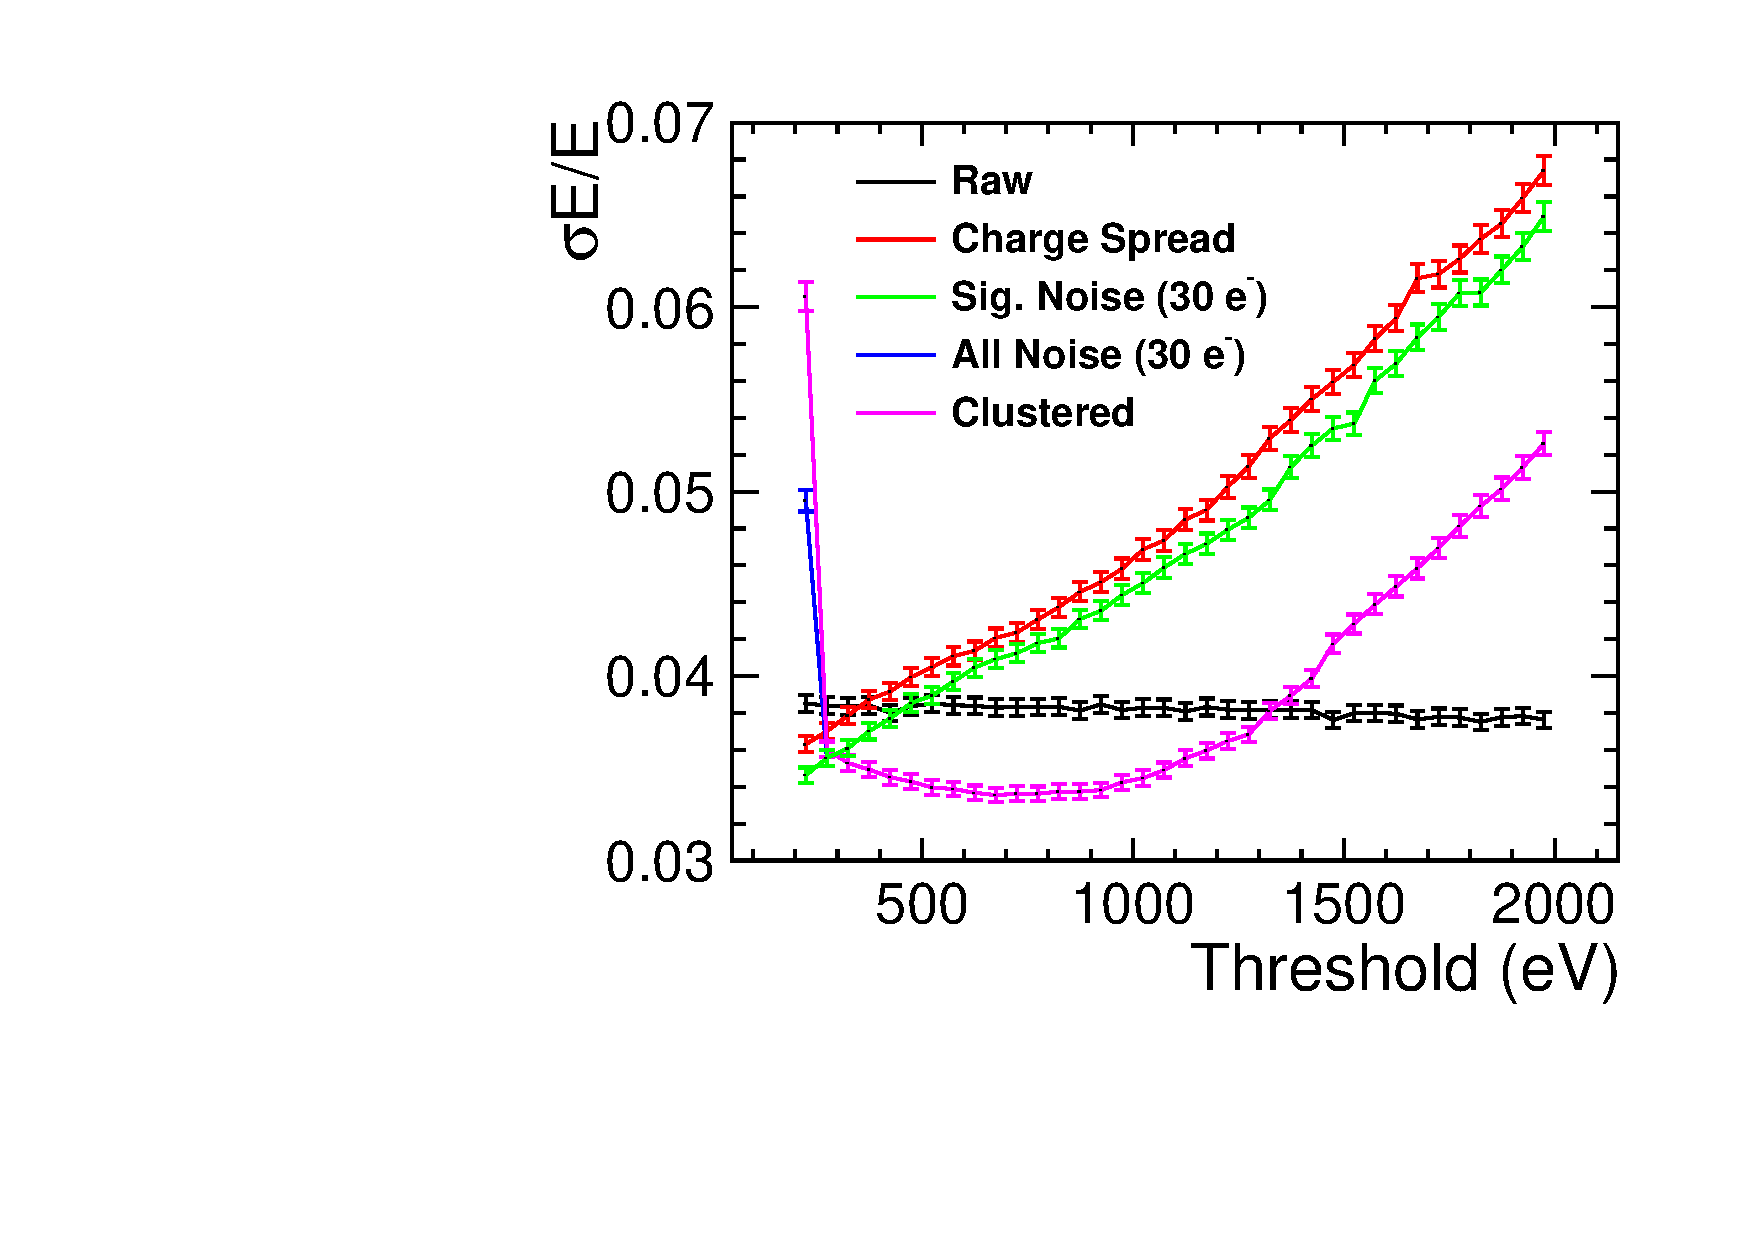
\includegraphics[width=0.7\textwidth,keepaspectratio]{DECALStudies/fig/ThresholdScan.pdf}
  \caption{Variation in the energy resolution as a function of the threshold applied after each DigiMAPS effect is added. The effects are added seqeuntially in the order displayed in the legend.}
  \label{fig:digimapseffects}
\end{figure}

To understand how the effect these different factors have on the energy resolution, the energy resolution for a specific pixel configuration and photon energy (50~$\mu$m pitch, 18~$\mu$m epi, 20 GeV photons) is plotted as a function of the threshold applied to the pixels after each additional level of realism is included. This is shown in \reffig{fig:digimapseffects}. In the most simplistic case with no effects added, one can see that the choice of threshold has little effect in the range examined as the threshold range is far below the peak in the landau, with only a small improvement seen for higher thresholds where the effect of boundary crossings is reduced. Adding charge spreading results in less energy being deposited in the pixel, effectively lowering the landau peak. As such, the resolution is seen to get worse as the threshold increases as a large proportion of the signal hits are being removed by the threshold. It is also possible that charge can diffuse into neighbouring pixels resulting in an increased number of fake hits and so a greater fluctuation on the number of pixels fired. The effect of noise is broken down into the cases where the noise is only added to genuine signal hits and where it is added to all pixels. One can see that adding noise to the signal hits results in an improved performance as less hits are lost due to the threshold. Including noise in all the pixels has little effect at higher thresholds as the threshold is above the energy generated by the noise and so no additional hits are being created. For very low thresholds, hits can be generated from the noise alone which results in a significantly worse resolution. Including dead space has the effect or making the resolution worse across all thresholds as it simply results in consistent undercounting of the number of hits in the detector. Adding clustering improves the resolution for all but the lowest thresholds (where the hits are dominated almost entirely by noise effects,) even providing better performance than the raw pixel counting with minimal realism. The broad optimal resolution range after clustering also shows that the detector should be relatively insensitive to threshold variations between pixel. The improved resolution performance is a result of the clustering removing additional hits caused by the charge spread or boundary crossings leading to the number of hits measured being a more consistent and accurate representation of the true number of pixels hit by the shower. Note that while this improvement is observed for the particular energy and pixel configuration shown above, it is expected that for wider pixels and higher energies, the clustering will ultimately result in the resolution getting worse as when the detector is close to saturation genuine hits will start to occur in adjacent cells and so the clustering will remove genuine hits. Ultimately this reduced performance might be avoidable in future by developing a more sophisticated clustering algorithm that uses pattern recognition to identify whether a hit is likely to be from an EM shower or just from noise.


\subsection{Pixel Design Optimization Revisited}

After the additional levels of realism have been included, it is important to evaluate the impact they have on the optimal pixel configuration. Note that the charge spread is not included here as the necessary sub-pixel simulations required as input for each pixel configuration do not exist. The resulting distributions for the stochastic, noise and constant terms are shown in  \reffigs{fig:stochastictermDigiClust}, \ref{fig:noisetermDigiClust} and \ref{fig:constanttermDigiClust}.

\begin{figure}
  \centering
  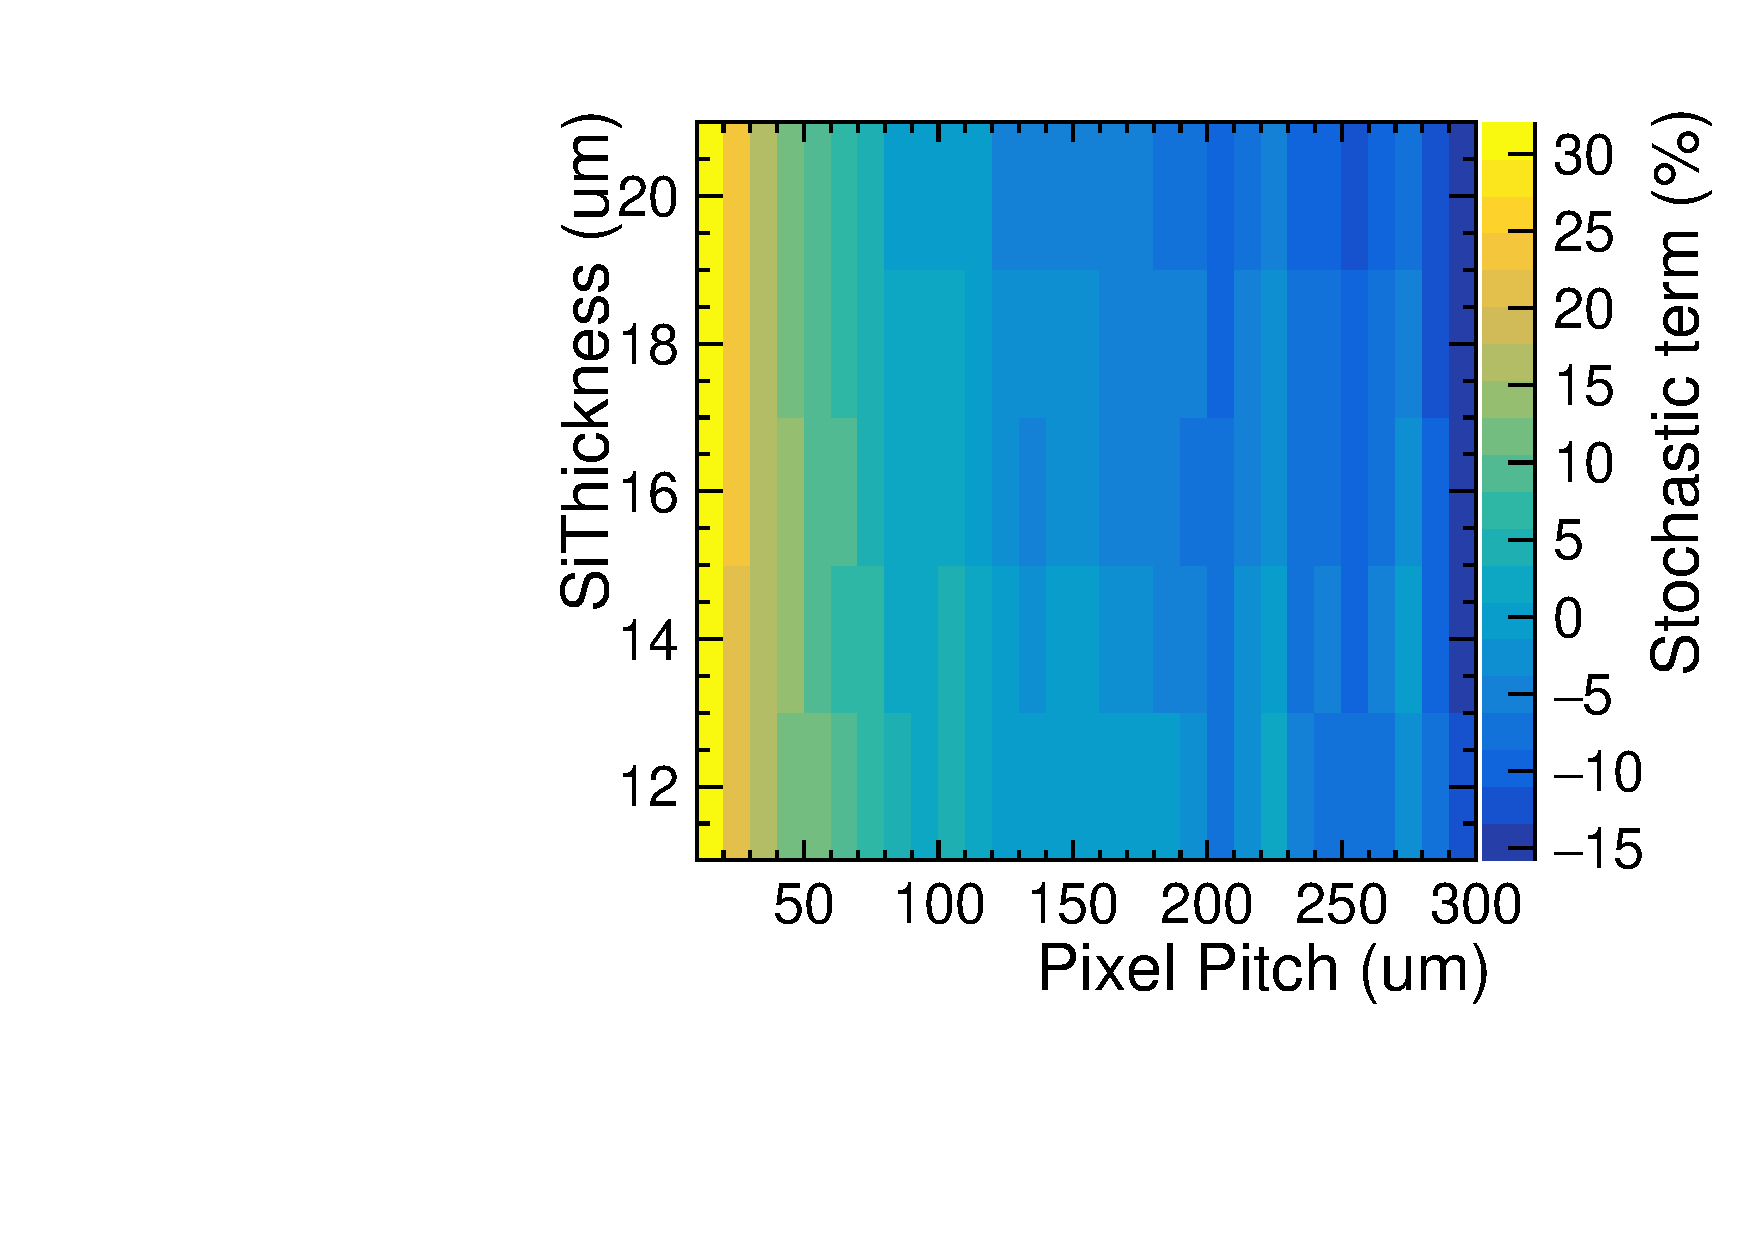
\includegraphics[width=0.7\textwidth,keepaspectratio]{DECALStudies/fig/FullDigiStochastic.pdf}
  \caption{Stochastic term of the energy resolution fits for all pixel configurations when including clustering, noise, dead space and threshold spread.}
  \label{fig:stochastictermDigiClust}
\end{figure}
\begin{figure}
  \centering
  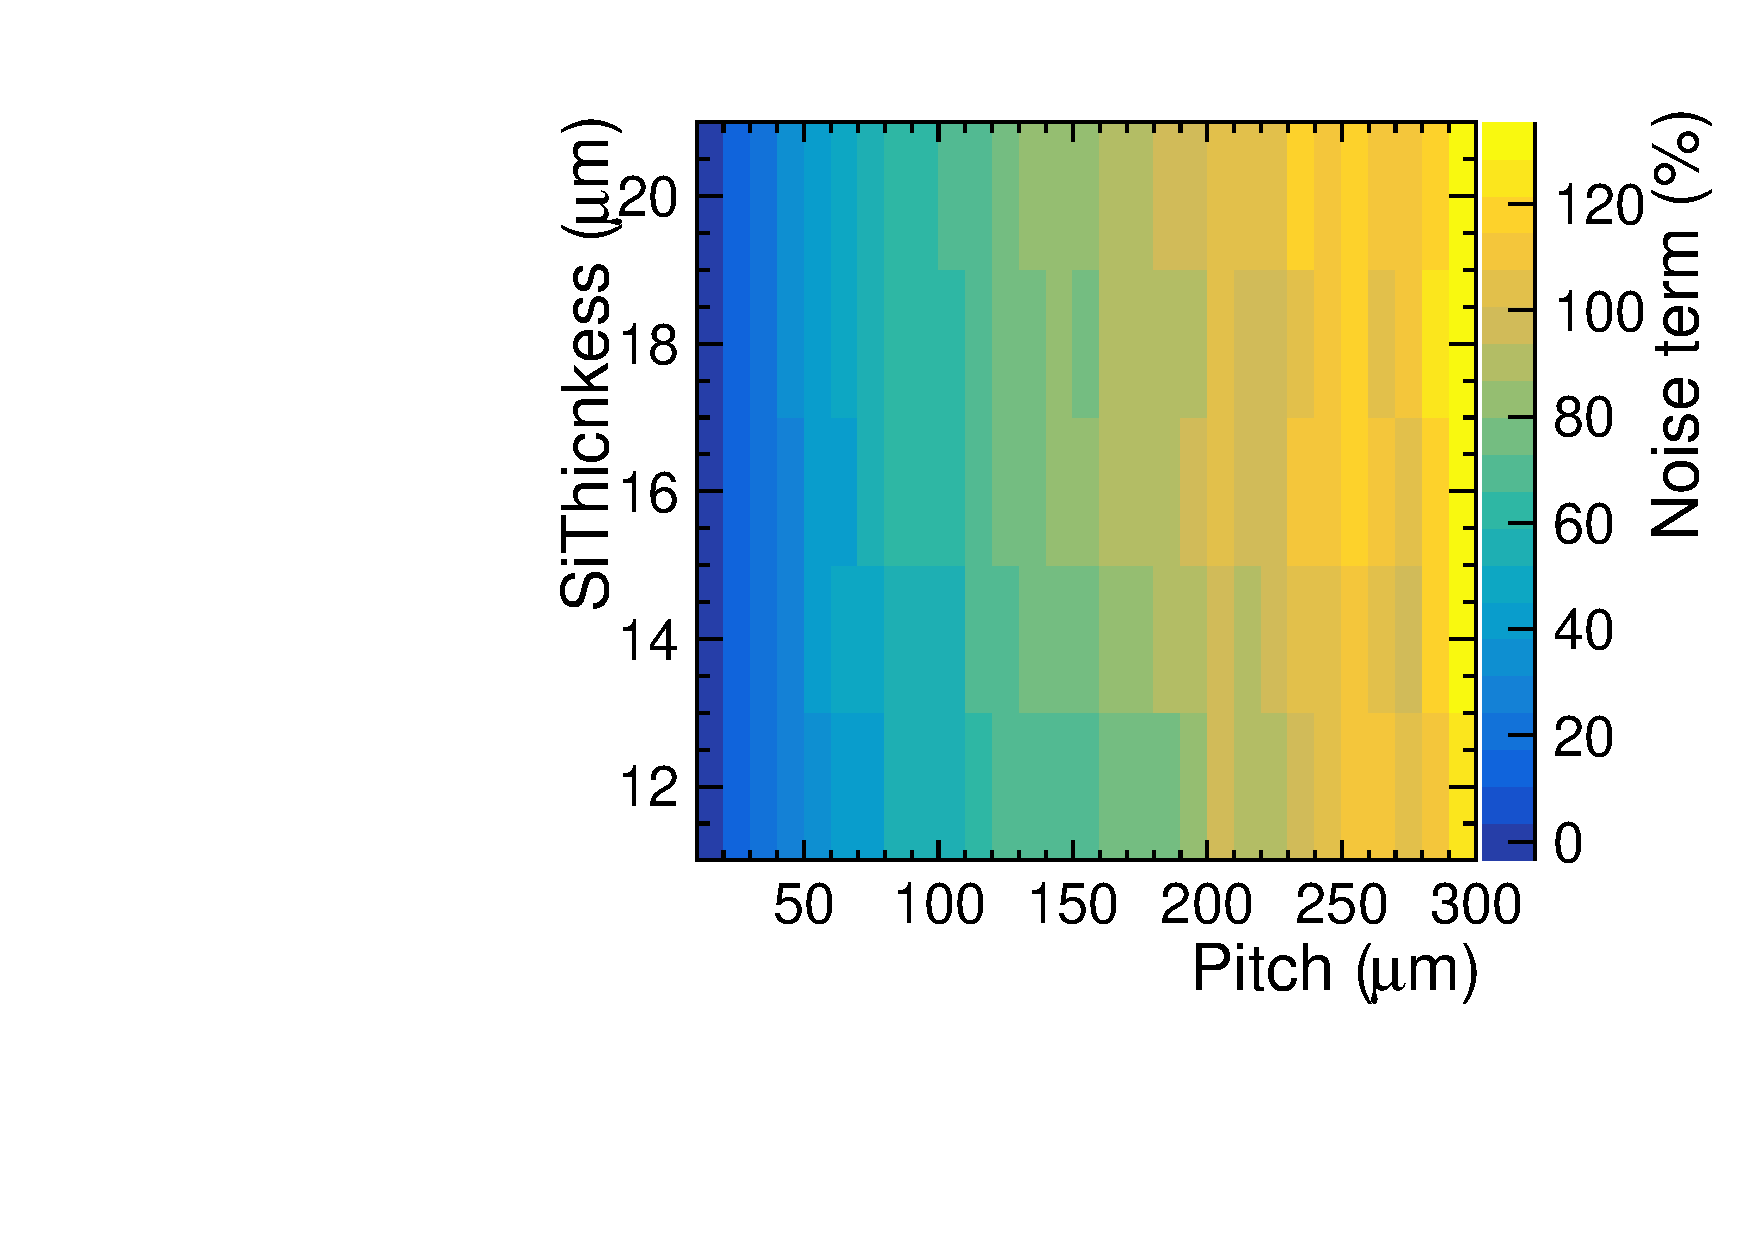
\includegraphics[width=0.7\textwidth,keepaspectratio]{DECALStudies/fig/FullDigiNoise.pdf}
  \caption{Noise term of the energy resolution fits for all pixel configurations when including clustering, noise, dead space and threshold spread.}
  \label{fig:noisetermDigiClust}
\end{figure}
\begin{figure}
  \centering
  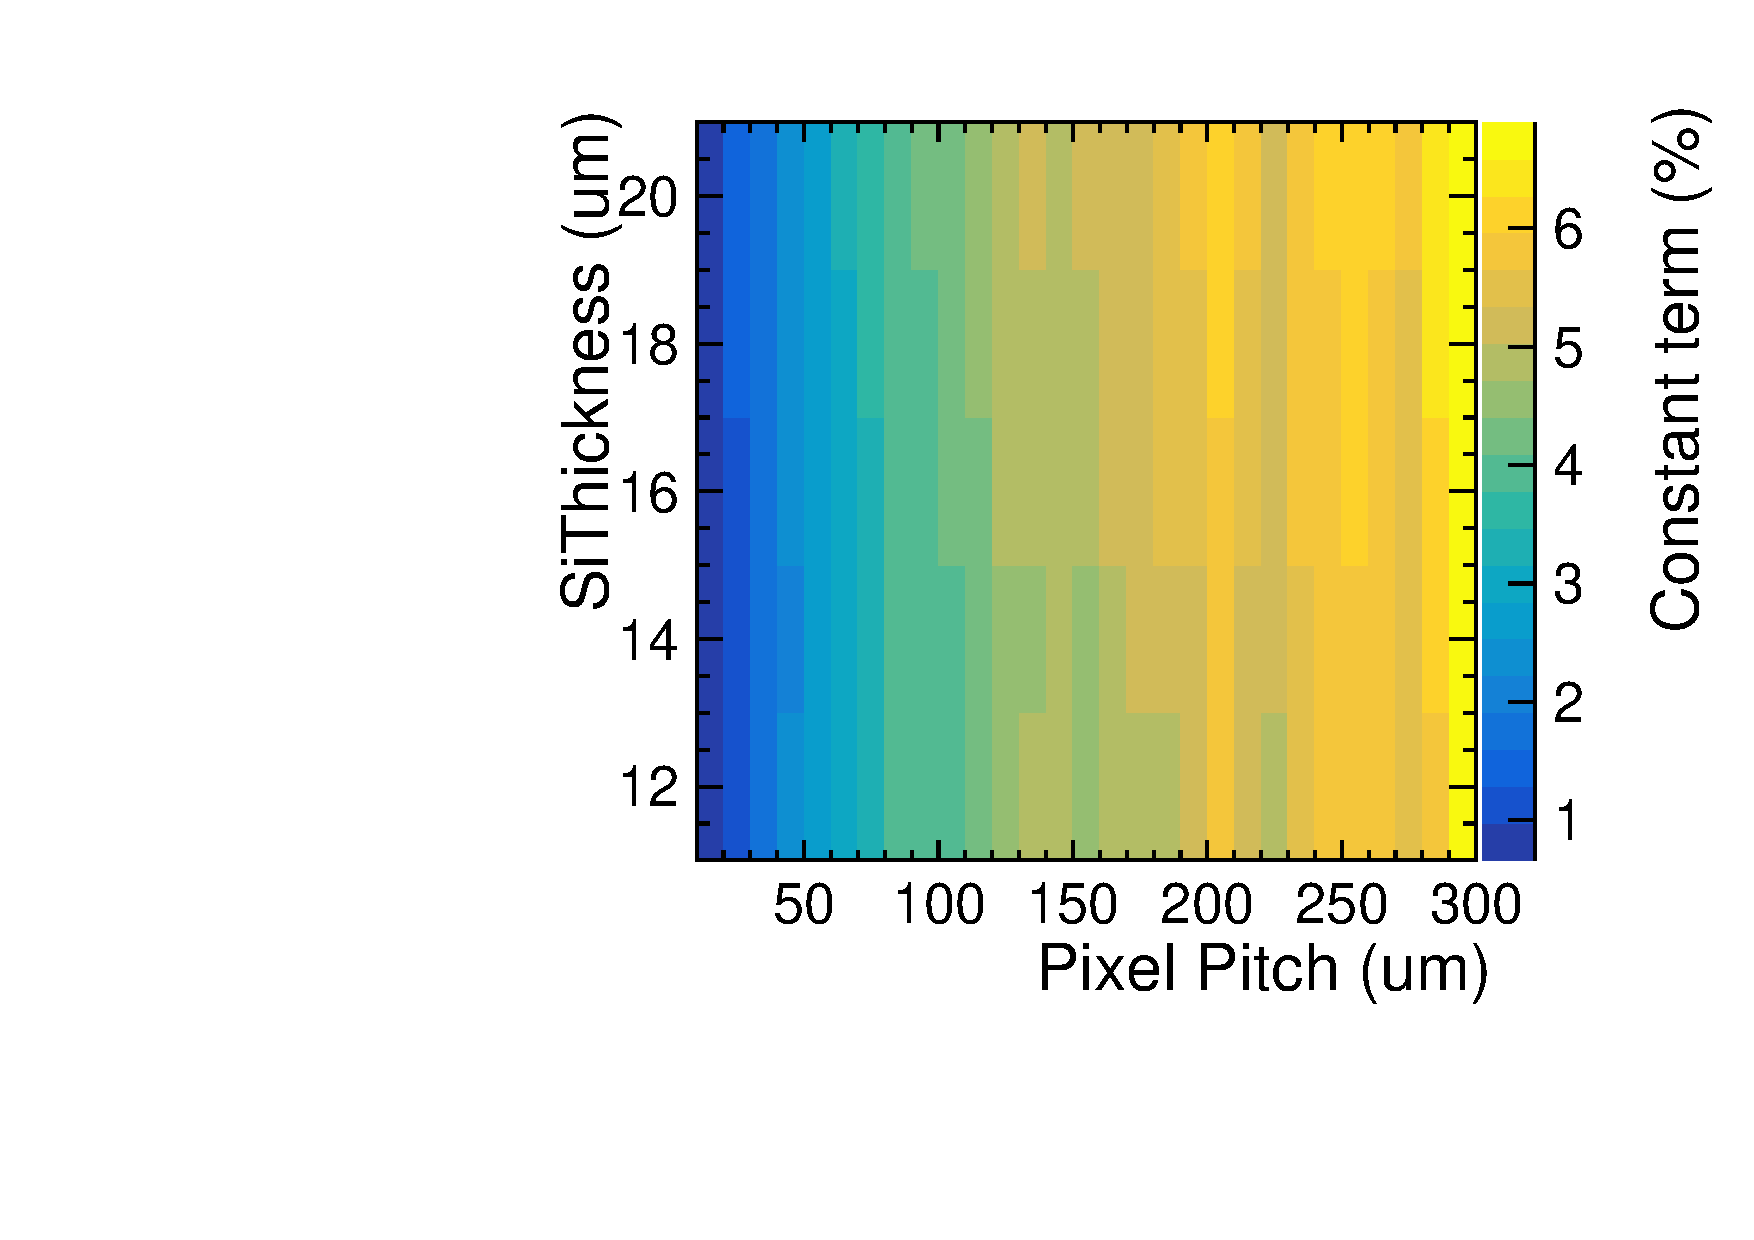
\includegraphics[width=0.7\textwidth,keepaspectratio]{DECALStudies/fig/FullDigiConstant.pdf}
  \caption{Constant term of the energy resolution fits for all pixel configurations when including clustering, noise, dead space and threshold spread. }
  \label{fig:constanttermDigiClust}
\end{figure}

\begin{figure}
  \centering
  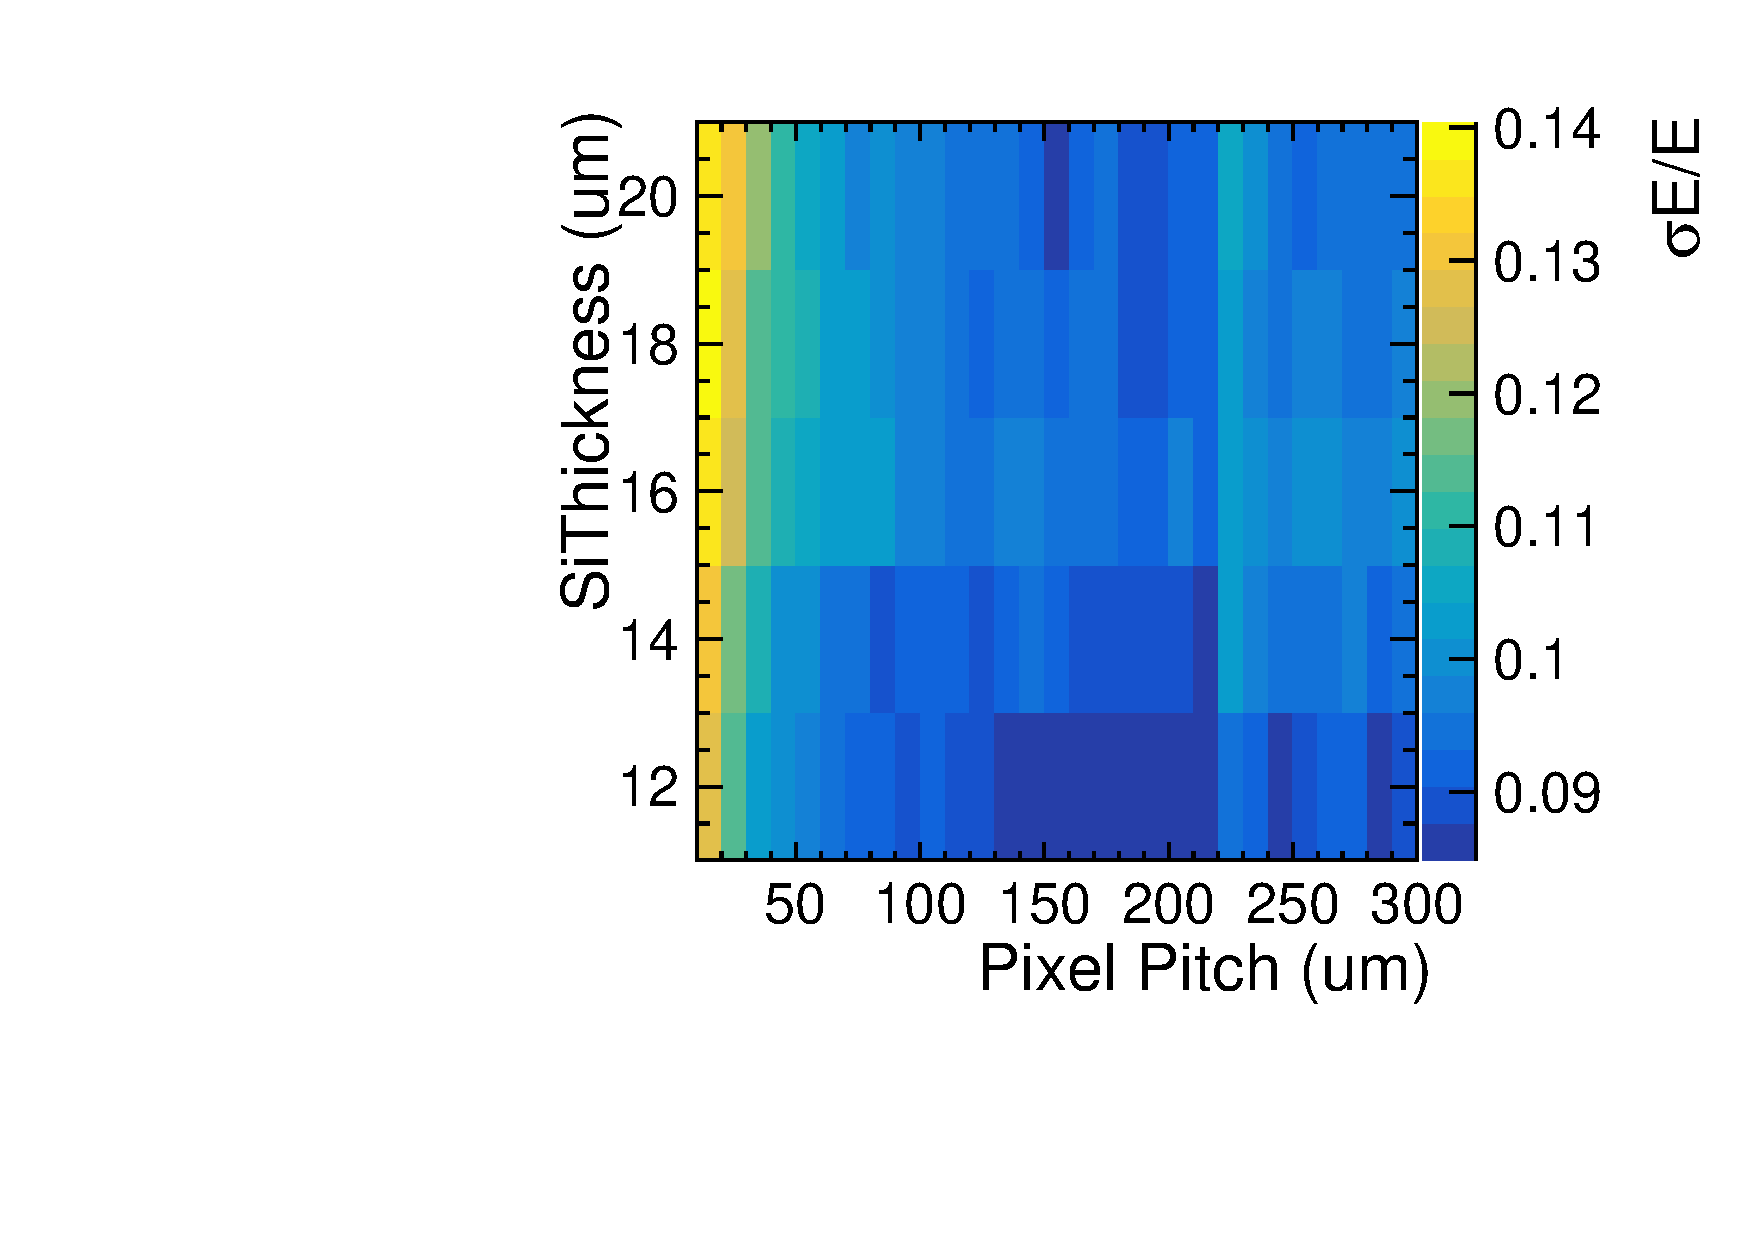
\includegraphics[width=0.7\textwidth,keepaspectratio]{DECALStudies/fig/NoClusterRes10.pdf}
  \caption{Energy resolution for 10 GeV photons after DigiMAPS is applied but without clustering.}
  \label{fig:resolution50DigiNoClust}
\end{figure}

Note that in some cases the resolution is seen to become negative, particluarly for wider pixel dimensions. This occurs when the resolution becomes so dominated by non linearities that the fit fails to accurately determine the resolution parameters. As such these regions are immediately ruled out as possible design choices.

\begin{figure}
  \centering
  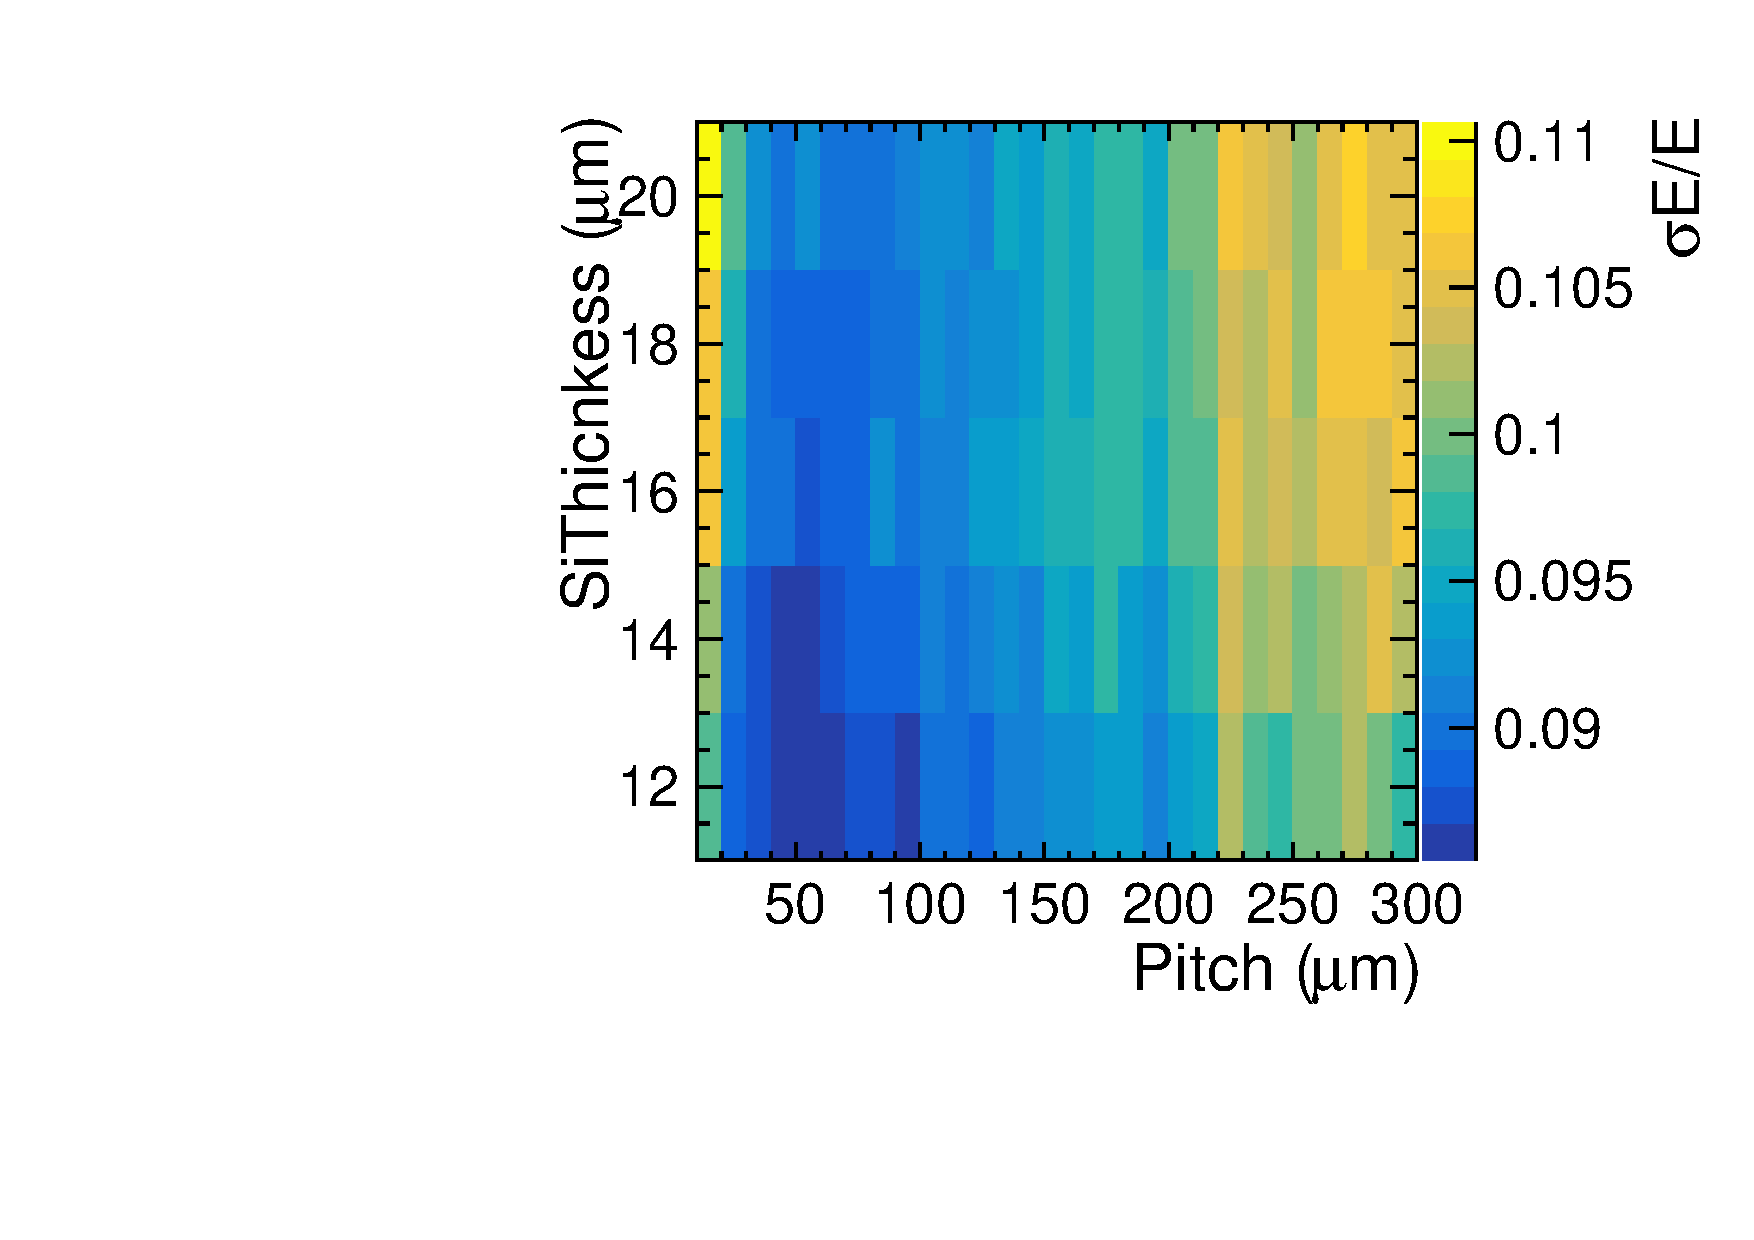
\includegraphics[width=0.7\textwidth,keepaspectratio]{DECALStudies/fig/FullDigiRes10.pdf}
  \caption{Energy resolution for 10 GeV photons after DigiMAPS is applied.}
  \label{fig:resolution10Digi}
\end{figure}

\begin{figure}
  \centering
  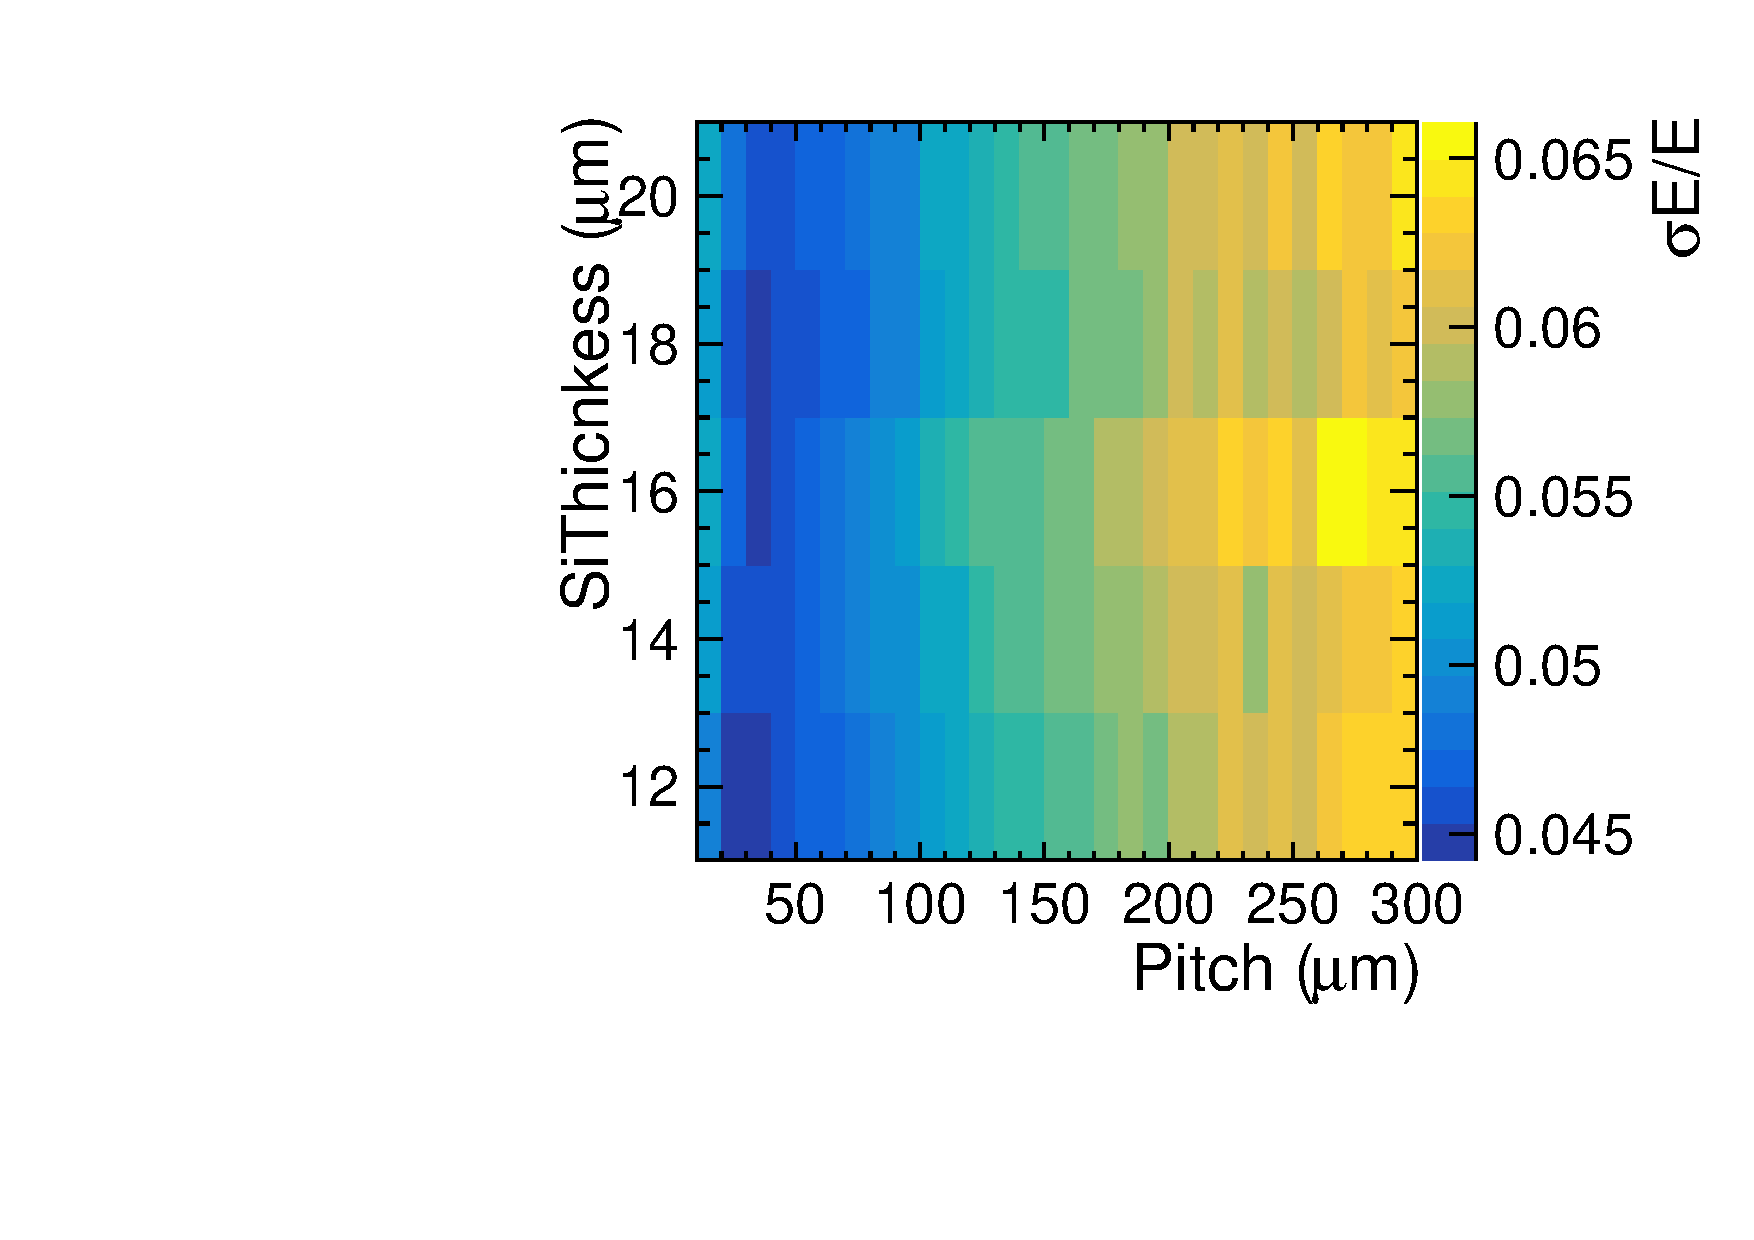
\includegraphics[width=0.7\textwidth,keepaspectratio]{DECALStudies/fig/FullDigiRes50.pdf}
  \caption{Energy resolution for 50 GeV photons after DigiMAPS is applied.}
  \label{fig:resolution50Digi}
\end{figure}

\begin{figure}
  \centering
  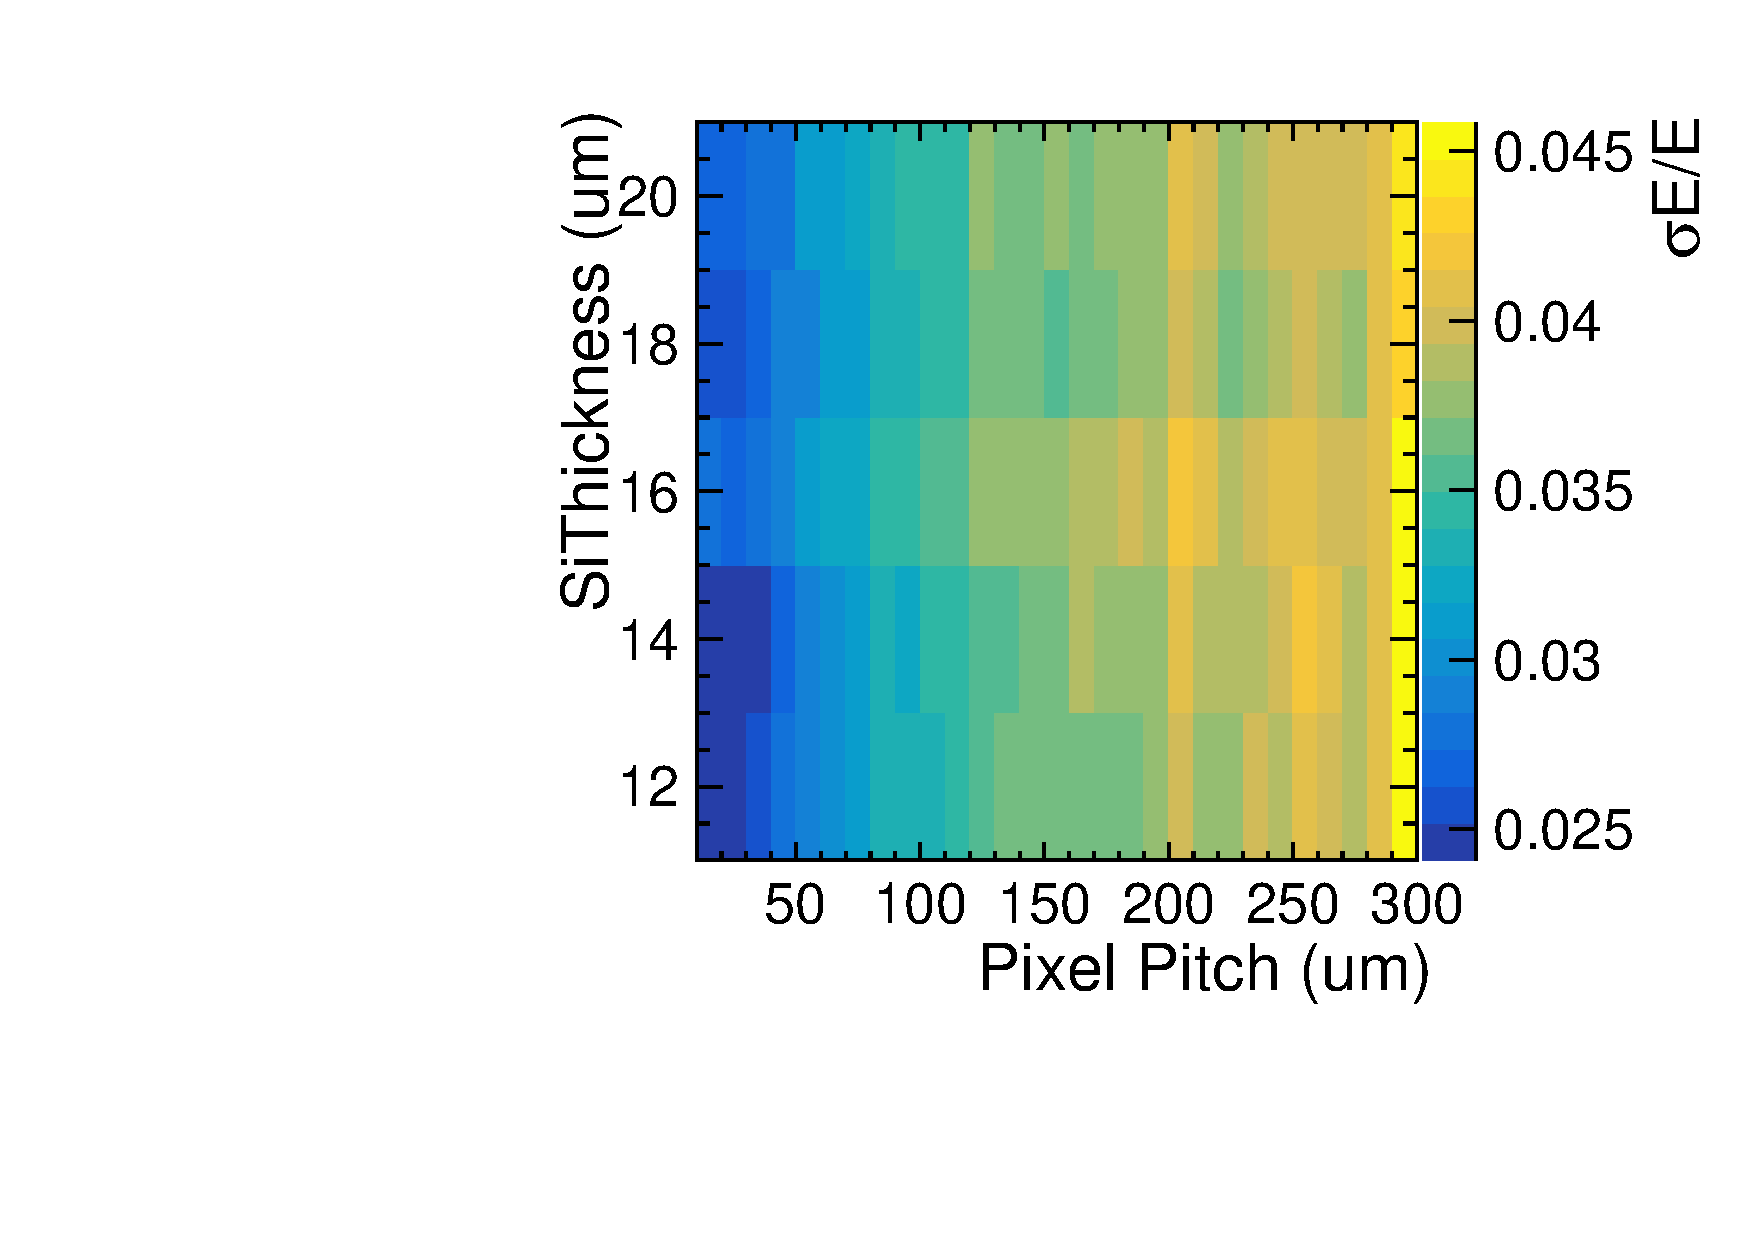
\includegraphics[width=0.7\textwidth,keepaspectratio]{DECALStudies/fig/FullDigiRes250.pdf}
  \caption{Energy resolution for 250 GeV photons after DigiMAPS is applied.}
  \label{fig:resolution250Digi}
\end{figure}

Again, to determine the optimal pixel configuration a relevant energy scale must be chosen as many of the effects controlling the resolution have a strong energy dependency. The resolution observed at the three working points of 10 GeV, 50 GeV and 250 GeV are shown in \reffigs{fig:resolution10Digi}, \ref{fig:resolution50Digi} and \ref{fig:resolution250Digi}. One can see that the net effect of including these effects is to shift the optimal resolution point to a narrower pixel pitch. This is predominantly a result of the clustering algorithm being included as highlighted by \reffig{fig:resolution50DigiNoClust} which shows the optimal resolution point at 10 GeV is relatively unchanged when including all DigiMAPS effects except the clustering. This is to be expected as in \reffig{fig:digimapseffects} it is observed that the effects other than clustering and charge spread approximately cancel each other out.

The shift in the optimal region when performing clustering is due to a combination of effects. Firstly the clustering will be helping to remove excess hits from boundary crossings which normally pushes the optimal point towards wider pixel pitches. Secondly, for wider pixels it is more likely that two adjacent pixels will have genuine contributions from the EM shower which can be merged by the clustering algorithm leading to undercounting. Both of these effects act to make the resolution better for narrower pixels and worse for wider pixels. One can see that at 250 GeV the optimal working point now corresponds to pixel ranges below what is considered within this study. For the typical energy scale for the \ac{ILC}, $\sim$50 GeV, the optimal pixel configuration is found to be at 30 $\mu m$ pitch, 12 $\mu m$ epi thickness as shown in \reffig{fig:resolution50Digi}. The resulting resolution is found to be:

\begin{equation}
  \frac{\sigma_E}{E}=\frac{16.1\%}{\sqrt{E}} \oplus \frac{0.5\%}{E} \oplus 0.4\%
\end{equation}

This is comparable to the performance observed for the analgue SiW equivalent proposed for \ac{ILD} which sees a resolution of (16.1$\pm$0.1) /$\sqrt{E(\text{GeV})} \oplus$(1.1$\pm$0.1)\% noting that the effect of charge spread has not been included here.


\section{Future Improvements}

While the studies here allow considerable progress to be made in designing a digital calorimeter, these is still much to be done to fully evaluate how it could perform as part of a full detector. In particular for simulation studies additional effects must be considered such as magnetic fields and angular depedencies. Currently all events are simulated with no magnetic field and with all particles entering the \ac{ECAL} at an angle of 90$^o$. This suppresses any angular dependence on the performance of the \ac{DECAL}. For example, the angle at which a particle enters the detector will change the amount of material traversed in both the absorber and active layers, effectively changing the number of interaction lengths a particle will see per layer. This can lead to miscounting of the number of particles passing through the detector. This is not as big an issue for analogue calorimeters where the energy of the hits are measured and scaled by a sampling fraction which is relatively insensitive to the angle of the incident particle. Regarding the magnetic field, additional complications can arise from low momentum particles being trapped between active layers and so not leaving sufficient hits in the detector, or from higher momentum particles being curved back into layers they have already traversed causing extra hits to be recorded.

Ideally the effect of charge spreading should be considered in performing the design optimization. As seen in \reffig{fig:digimapseffects} this can cause a large effect on the energy resolution however this had to be ignored in the optimization studies due to the inability to perform the necessary sub pixel simulations with DigiMAPS. However examining the effect of charge spread would require a dedicated optimization study of it's own as there are multiple diode configurations which could be used with the optimal diode layout ultimately depending on the pixel dimensions itself. As such it makes more sense to settle on an optimal pixel geometry first and then design the pixel substructure to maximise the charge collection efficiency for this geometry.

In the longer term the ultimate aim will be to implement the \ac{DECAL} into the particle flow algorithms used for \ac{ILD}. At the beginning of this chapter it was postulated that the higher granularity of the \ac{DECAL} could improve particle flow performance however without implementing this the scale of any imporvements cannot be known.

It should also be noted that the studies presented here are still only using an adaptation of the existing \ac{ILD} analogue \ac{ECAL} design. It is unlikely that this represents the optimal design for a digital calorimeter. In particular, a \ac{DECAL} might benefit from chaging the absorbing material to one with a larger Moliere radius to produce a less dense shower and so less saturation. While this should provide a better single particle resolution, it may result in a worse jet resolution as showers could start to overlap. As such, further study is required to find the optimal material choices for a \ac{DECAL}.



\section{Conclusion}

Here we have examined the potential for implementing a digital calorimeter within the \ac{ILD} geometry by studying the single particle energy resolution for various pixel pitches and epitaxial thicknesses. Initially studies were performed by simplying measuring raw energy deposits within the calorimeter as determined by GEANT4. This allowed the two main driving factors for optimizing the pixel configuration to be indentified. For 
